\section{Introduction}\label{sec:intro}

Some treatments must work on several targets at once. A quadrivalent meningococcal conjugate vaccine is licensed on immunogenicity against each of serogroups A, C, W and Y, and a confirmatory trial succeeds only if the vaccine is non-inferior to the licensed comparator on all four \citep{yang2024,ostergaard2009}. Such endpoints are co-primary. Each is tested at level $\alpha$, and success is declared only if every test rejects \citep{berger1982}. No multiplicity adjustment is needed, but the power of the conjunction is at most the smallest marginal power and falls well below it when the endpoints are weakly correlated. The sample size therefore rises with the number of endpoints \citep{offen2007,chuangstein2007,sozu2010,hamasaki2018}.

When several candidate doses or formulations precede the confirmatory trial, an adaptive seamless phase II/III design combines selection and confirmation \citep{bauer1994,stallard2003,posch2005,bretz2006,jennison2007,stallard2011}. Stage 1 randomises subjects to all candidates and control, and an interim analysis selects one candidate. Stage 2 continues with the selected candidate and control, and the final analysis uses the data of both stages. A combination test over stages and a closed test over candidates control the type I error under data-dependent selection \citep{marcus1976,hommel2001}. Regulators now ask sponsors to select the dose before confirmation \citep{fda2024}, and seamless designs for this purpose have followed \citep{li2024,liu2026}. \citet{yang2024} proposed a Bayesian seamless design for co-primary endpoints that applies the co-primary criterion to every candidate at the interim and sets the stage-2 sample size by predictive power.

With co-primary endpoints the cost of the conjunction is paid at the interim as well as at the final analysis, once for each candidate. Ranking candidates on the co-primary criterion ranks them on their weakest endpoint. At the sample sizes of a selection stage the weakest endpoint is a noisy statistic, and it ignores the other endpoints. We ask whether the interim can rank the candidates on a criterion that pools the endpoints while the final claim stays co-primary.

Seamless designs already select on one endpoint and confirm on another. Short-term or surrogate endpoints have been used to select treatments that are confirmed on a long-term endpoint \citep{stallard2010,friede2011,kunz2014}, and progression-free survival has been used to select a subpopulation that is confirmed on overall survival \citep{jenkins2011}. In those designs the selection endpoint is observed earlier. Here both criteria use the same $K$ binary responses of the same subjects. Selection uses a pre-specified weighted composite, the weighted responder score of \citet{zaslavsky2013}, and confirmation uses the co-primary criterion. The composite and the endpoint success probabilities are linear in the probabilities of the $2^K$ response patterns, so one Dirichlet--multinomial model \citep{thall1995,yang2024} gives the posterior of every quantity used at the interim. Selection is Bayesian and confirmation is a frequentist test.

The paper makes three contributions. Section~\ref{sec:design} defines the design and proves that the probability of a false co-primary claim is at most $\alpha$ for any selection rule, futility rule and stage-2 sample size (Theorem~\ref{thm:t1e}). The final analysis is a closed test over all dose--endpoint hypotheses. Closing each endpoint separately over doses fails when different doses fail on different endpoints, and its false-claim rate reached $0.055$ at $\alpha=0.025$ in our simulations. Section~\ref{sec:saving} gives the conditions under which the composite needs a smaller stage 1 than the co-primary criterion for the same probability of correct selection, and the cases in which it needs a larger one. Section~\ref{sec:sim} compares the two designs by simulation from selection to final claim and derives a rule for choosing between them. R code that reproduces every table and figure is available.

\section{Motivating example}\label{sec:motivation}

\citet{yang2024} describe a trial of a quadrivalent meningococcal tetanus toxoid-conjugate vaccine (MenACWY-TT). Seroresponse to each of serogroups A, C, W and Y was a co-primary endpoint, and success required non-inferiority to the licensed comparator on all four with a margin of $-10$ percentage points. The comparator seroresponse rates were $0.425$, $0.497$, $0.448$ and $0.434$.

A formulation-selection study preceded trials of this kind. \citet{ostergaard2009} compared five candidate MenACWY-TT formulations, which differed in polysaccharide content and conjugation method, with a licensed ACWY polysaccharide vaccine in two open-label studies of 50 adults aged 18--25 and 125 adolescents aged 15--19. The immunogenicity endpoints were the percentages of serum bactericidal antibody responders to serogroups A, C, W-135 and Y. Responder percentages did not differ from control for any formulation on any serogroup, except that serogroup A was lower after one formulation. The selection problem thus had $M=5$ candidates, $K=4$ binary endpoints and a concurrent control, and it was decided on 25--35 subjects per arm.

Two features of this setting suit a composite at the selection stage. The endpoints are positively dependent, because they are responses of the same immune system to conjugates of the same carrier, and a better formulation tends to be better on every serogroup. A weighted sum of the four responder rates then carries most of the information that separates formulations. The endpoints also have a clinical weighting, because serogroup-specific disease burden differs by age and region, so the weights can be fixed from epidemiological data before the trial. A seamless design would randomise the candidates and control in stage 1, select on the composite, continue the selected formulation and control into stage 2, and confirm on the four co-primary endpoints with the stage-1 data included.

The serogroup A shortfall shows the weakness of a composite. One endpoint failed and three responded, and a weighted average of four responder rates changes little when one of them falls. Section~\ref{sec:stage1} adds a per-endpoint futility check for this case.

\section{The design}\label{sec:design}

\subsection{Setting and notation}

Consider a randomised two-stage trial that compares $M$ doses $a=1,\dots,M$ of an experimental agent with a concurrent control, arm $0$, on $K$ binary endpoints. We say doses, but the arms are unordered. No dose--response structure is used, and the design applies unchanged to formulations or distinct treatments. Stage 1 randomises $n_1$ subjects to each of the $M+1$ arms. The interim analysis selects at most one dose $a^\star$. Stage 2 randomises $n_2$ subjects to each of $a^\star$ and control, and the final analysis uses both stages. The planned per-arm total on $a^\star$ and control is $n_{\mathrm{tot}}=n_1+n_2$. Figure~\ref{fig:schematic} shows the trial flow and the model.

\begin{figure}
\centering
\resizebox{\textwidth}{!}{%% Schematic of the design (Figure 1). Input from body.tex; requires tikz with
%% libraries positioning, arrows.meta, shapes.geometric, fit, calc (loaded in main.tex).
\begin{tikzpicture}[
  font=\footnotesize,
  >={Stealth[length=1.8mm]},
  arm/.style={draw, rounded corners=1.5pt, minimum width=14mm, minimum height=6.5mm,
              align=center, fill=black!6, inner sep=2pt},
  blk/.style={draw, rounded corners=1.5pt, align=center, inner sep=4pt, text width=62mm, fill=white},
  gate/.style={draw, diamond, aspect=2.6, align=center, inner sep=1pt, fill=black!3},
  lab/.style={font=\footnotesize\itshape, text=black!65},
  ptitle/.style={font=\footnotesize\bfseries, text=black!75},
  pat/.style={draw, minimum width=11mm, minimum height=6mm, inner sep=1pt, font=\scriptsize, align=center},
  fun/.style={draw, rounded corners=1.5pt, align=center, inner sep=3pt, font=\scriptsize, text width=34mm},
]
%% ---------------------------------------------------------------- panel (a)
\node[ptitle, anchor=west] (pa) at (0,0) {(a) Trial flow};
% stage 1 arms
\node[arm, below=8mm of pa.west, anchor=north west, xshift=4mm] (d1) {Dose 1\\ $n_1$};
\node[arm, right=2mm of d1] (d2) {Dose 2\\ $n_1$};
\node[right=1mm of d2, font=\small] (dots) {$\cdots$};
\node[arm, right=1mm of dots] (dM) {Dose $M$\\ $n_1$};
\node[arm, right=2mm of dM, fill=black!12] (c1) {Control\\ $n_1$};
\node[lab, above=0.8mm of d1.north west, anchor=south west, xshift=-1mm] {Stage 1: randomise $n_1$ subjects to each of $M+1$ arms};
% posterior
\node[blk, below=7mm of $(d1.south)!0.5!(c1.south)$] (post)
  {Dirichlet--multinomial posterior for each arm,\\
   $\bpi_a\mid\bx_a\sim\Dir(\bkappa_a+\bx_a)$,\\
   exact moments of $S_a$ and of every $p_{a,k}$ (Appendix~A)};
% composite gate
\node[blk, below=4mm of post] (comp)
  {\textbf{Selection on the composite}\\
   $G_a=\Pr\big(S_a-S_0>\gamma\mid\bx\big)$,\quad $a^\star=\arg\max_a G_a$};
\node[gate, below=4mm of comp] (dec) {$G_{a^\star}\ge\eta$?};
\node[blk, text width=22mm, right=6mm of dec, fill=black!6] (stop) {Stop for\\ futility};
% stage 2 arms
\node[arm, below=13mm of dec, xshift=-9mm] (a2) {Dose $a^\star$\\ $n_2$};
\node[arm, right=2mm of a2, fill=black!12] (c2) {Control\\ $n_2$};
\node[lab, above=0.8mm of a2.north west, anchor=south west, xshift=-12mm] {Stage 2: randomise $n_2$ subjects to $a^\star$ and control};
% final analysis
\node[blk, below=5mm of $(a2.south)!0.5!(c2.south)$] (fin)
  {\textbf{Confirmation on the co-primary endpoints}\\
   closed test over all $MK$ dose--endpoint hypotheses $H_{a,k}$:\\
   Simes-combined stage-1 and stage-2 $p$-values for each intersection,\\
   combined across stages by the inverse-normal rule};
\node[blk, below=4mm of fin, fill=black!3] (claim)
  {Claim for $a^\star$ if $H_{a^\star,k}$ is rejected for every $k=1,\dots,K$\\
   (Theorem~1 bounds the false-claim rate by $\alpha$ for every configuration)};
% arrows
\foreach \n in {d1,d2,dM,c1} \draw[->] (\n.south) -- ($(\n.south |- post.north)$);
\draw[->] (post) -- (comp);
\draw[->] (comp) -- (dec);
\draw[->] (dec) -- node[above, lab] {no} (stop);
\draw[->] (dec) -- node[right, lab, pos=0.35] {yes} ($(dec.south)+(0,-4.5mm)$) -| (a2.north);
\draw[->] ($(dec.south)+(0,-4.5mm)$) -| (c2.north);
\foreach \n in {a2,c2} \draw[->] (\n.south) -- ($(\n.south |- fin.north)$);
\draw[->] (fin) -- (claim);
% stage-1 data re-used
\coordinate (ru) at ($(post.east)+(20mm,0)$);
\draw[->, dashed] (post.east) -- (ru) -- (ru |- fin.east) -- (fin.east);
\node[lab, align=right, anchor=east] at ($(ru |- a2.east)+(-1.5mm,0)$) {stage-1 data of $a^\star$\\ and control enter\\ the final analysis};
%% ---------------------------------------------------------------- panel (b)
\begin{scope}[xshift=104mm]
\node[ptitle, anchor=west] (pb) at (0,0) {(b) One cell-probability vector, two functionals ($K=3$)};
\node[lab, below=4mm of pb.west, anchor=north west, text width=86mm] (btxt)
  {Each subject falls in one of $J=2^K$ response patterns. The success probability $p_{a,k}$ used for confirmation is the
   sum of $\bpi_a$ over the cells $\cR_k$ in which endpoint $k$ succeeds (dots in row $k$). The composite used for selection
   is the sum with weights $c_j(\bw)=\sum_k w_k\ind_{\cR_k}(j)$, the weighted column sums of the dot rows. One posterior serves both stages, and the dependence between
   endpoints is carried by the shared cells.};
% the J = 8 cells, ordered as j = 1 + y_1 + 2 y_2 + 4 y_3
\node[pat, minimum width=7mm, below=5mm of btxt.south west, anchor=north west, xshift=28mm] (c1) {$000$\\ $\pi_{a,1}$};
\node[pat, minimum width=7mm, right=1mm of c1] (c2) {$100$\\ $\pi_{a,2}$};
\node[pat, minimum width=7mm, right=1mm of c2] (c3) {$010$\\ $\pi_{a,3}$};
\node[pat, minimum width=7mm, right=1mm of c3] (c4) {$110$\\ $\pi_{a,4}$};
\node[pat, minimum width=7mm, right=1mm of c4] (c5) {$001$\\ $\pi_{a,5}$};
\node[pat, minimum width=7mm, right=1mm of c5] (c6) {$101$\\ $\pi_{a,6}$};
\node[pat, minimum width=7mm, right=1mm of c6] (c7) {$011$\\ $\pi_{a,7}$};
\node[pat, minimum width=7mm, right=1mm of c7] (c8) {$111$\\ $\pi_{a,8}$};
\node[lab, above=0.5mm of c1.north west, anchor=south west] {cells $y_1y_2y_3$ with probabilities $\pi_{a,j}$};
% membership rows: a dot where component k succeeds in cell j
\coordinate (r1) at ($(c1.south)+(0,-3.2mm)$);
\coordinate (r2) at ($(c1.south)+(0,-6.6mm)$);
\coordinate (r3) at ($(c1.south)+(0,-10.0mm)$);
\coordinate (rc) at ($(c1.south)+(0,-14.6mm)$);
\foreach \j/\m in {1/0,2/1,3/0,4/1,5/0,6/1,7/0,8/1}
  {\ifnum\m=1 \fill (c\j |- r1) circle (0.75mm); \else \fill[black!25] (c\j |- r1) circle (0.3mm); \fi}
\foreach \j/\m in {1/0,2/0,3/1,4/1,5/0,6/0,7/1,8/1}
  {\ifnum\m=1 \fill (c\j |- r2) circle (0.75mm); \else \fill[black!25] (c\j |- r2) circle (0.3mm); \fi}
\foreach \j/\m in {1/0,2/0,3/0,4/0,5/1,6/1,7/1,8/1}
  {\ifnum\m=1 \fill (c\j |- r3) circle (0.75mm); \else \fill[black!25] (c\j |- r3) circle (0.3mm); \fi}
\node[font=\scriptsize, anchor=east] at ($(c1.west |- r1)+(-1.5mm,0)$) {$p_{a,1}=\pi_a(\cR_1)$};
\node[font=\scriptsize, anchor=east] at ($(c1.west |- r2)+(-1.5mm,0)$) {$p_{a,2}=\pi_a(\cR_2)$};
\node[font=\scriptsize, anchor=east] at ($(c1.west |- r3)+(-1.5mm,0)$) {$p_{a,3}=\pi_a(\cR_3)$};
% composite weights c_j(w): the weighted column sums of the dot rows
\node[font=\scriptsize, anchor=east] at ($(c1.west |- rc)+(-1.5mm,0)$) {$c_j(\bw)$};
\node[font=\tiny, align=center] at (c1 |- rc) {$0$};
\node[font=\tiny, align=center] at (c2 |- rc) {$w_1$};
\node[font=\tiny, align=center] at (c3 |- rc) {$w_2$};
\node[font=\tiny, align=center] at (c4 |- rc) {$w_1{+}w_2$};
\node[font=\tiny, align=center] at (c5 |- rc) {$w_3$};
\node[font=\tiny, align=center] at (c6 |- rc) {$w_1{+}w_3$};
\node[font=\tiny, align=center] at (c7 |- rc) {$w_2{+}w_3$};
\node[font=\tiny, align=center] at (c8 |- rc) {$w_1{+}w_2$\\ ${}+w_3$};
\draw[black!40] ($(c1.west |- rc)+(0,2.3mm)$) -- ($(c8.east |- rc)+(0,2.3mm)$);
% selection and confirmation
\coordinate (mid) at ($(c4.east)!0.5!(c5.west)$);
\coordinate (sN) at ($(mid |- rc)+(0,-6.5mm)$);
\node[fun, text width=60mm, anchor=north] (S) at (sN)
  {\textbf{Selection:} $S_a=\sum_k w_kp_{a,k}=\bc(\bw)^\top\bpi_a$\\ one scalar contrast $S_a-S_0$ per dose};
\node[fun, below=3.5mm of S, text width=60mm, fill=black!3] (CP)
  {\textbf{Confirmation:} $p_{a^\star,k}-p_{0,k}>\delta_k$ for every $k$\\ (co-primary, closed test over doses and endpoints)};
\draw[->] ($(mid |- rc)+(0,-2.8mm)$) -- (S.north);
\draw[dashed] ($(c8.east |- r1)+(3mm,0)$) -- ($(c8.east |- r3)+(3mm,0)$);
\draw[->, dashed] ($(c8.east |- r3)+(3mm,0)$) |- (CP.east);
\end{scope}
\end{tikzpicture}
}
\caption{The design: (a) trial flow and (b) the cell-probability model that links the composite and the co-primary criterion, drawn for $K=3$ endpoints.}\label{fig:schematic}
\end{figure}

A subject's response is $\bY=(Y_1,\dots,Y_K)\in\{0,1\}^K$. The $J=2^K$ response patterns define multinomial cells with probabilities $\bpi_a=(\pi_{a,1},\dots,\pi_{a,J})$ in arm $a\in\{0,1,\dots,M\}$. For a set of cells $\cR$ write $\pi_a(\cR)=\sum_{j\in\cR}\pi_{a,j}$. Let $\cR_k$ be the set of cells in which endpoint $k$ is a success. The success probability of endpoint $k$ is $p_{a,k}=\pi_a(\cR_k)$, the effect of dose $a$ is $\theta_{a,k}=p_{a,k}-p_{0,k}$, and $\delta_k\le0$ is the margin, negative for non-inferiority and zero for superiority.

\subsection{Probability model}\label{sec:model}

Following \citet{thall1995} and \citet{yang2024}, the cell probabilities of each arm have a Dirichlet prior, $\bpi_a\sim\Dir(\bkappa_a)$ with total mass $m_a=\sum_j\kappa_{a,j}$, and the cell counts of each stage are multinomial. Let $\bx_a$ be the stage-1 cell counts of arm $a$ and $\bx$ the stage-1 data of all arms. The posterior is $\bpi_a\mid\bx_a\sim\Dir(\bkappa_a+\bx_a)$, with mean $\hat\bpi_a=(\bkappa_a+\bx_a)/(m_a+n_1)$. By the aggregation property of the Dirichlet distribution (Appendix~\ref{app:dirichlet}), for any set of cells $\cR$,
\begin{equation}\label{eq:beta}
\pi_a(\cR)\mid\bx_a\sim\Beta\big((m_a+n_1)\,\hat\pi_a(\cR),\ (m_a+n_1)\{1-\hat\pi_a(\cR)\}\big).
\end{equation}
Each $p_{a,k}$ therefore has a Beta posterior with mean $\hat p_{a,k}=\hat\pi_a(\cR_k)$. The posterior dependence between $p_{a,k}$ and $p_{a,k'}$ comes from the cells they share, $\cR_k\cap\cR_{k'}$, and the model needs no separate correlation parameter. We use the prior $\bkappa_a=\mathbf 1/J$, which carries the weight of one observation per arm. Section~\ref{sec:prior} examines stronger and arm-specific priors.

\subsection{Stage 1: selection on a weighted composite}\label{sec:stage1}

Each endpoint has a clinical weight $w_k\ge0$ with $\sum_kw_k=1$ \citep{zaslavsky2013}. The composite of arm $a$ is the expected weighted score of a subject,
\begin{equation}\label{eq:composite}
S_a=\E\Big[\sum_{k=1}^K w_kY_k\,\Big|\,a\Big]=\sum_{k=1}^K w_k\,p_{a,k}=\bc(\bw)^\top\bpi_a,\qquad
\bc(\bw)=\sum_{k=1}^K w_k\,\ind_{\cR_k},
\end{equation}
where $\ind_{\cR_k}$ is the $J$-vector that indicates the cells in $\cR_k$. The composite is linear in $\bpi_a$, and its contrast with control is $\Delta_a=S_a-S_0$. Its posterior moments are (Appendix~\ref{app:dirichlet})
\begin{equation}\label{eq:moments}
\E[S_a\mid\bx_a]=\sum_{k=1}^K w_k\,\hat p_{a,k},\qquad
\Var[S_a\mid\bx_a]=\frac{1}{m_a+n_1+1}\sum_{k=1}^K\sum_{k'=1}^K w_kw_{k'}\big(\hat p_{a,kk'}-\hat p_{a,k}\,\hat p_{a,k'}\big),
\end{equation}
where $\hat p_{a,kk'}=\hat\pi_a(\cR_k\cap\cR_{k'})$ is the posterior mean of the probability that endpoints $k$ and $k'$ both succeed. We approximate the posterior of $\Delta_a$, and of each endpoint contrast $p_{a,k}-p_{0,k}$, by a normal distribution with the exact posterior mean and variance. With the weak prior the resulting posterior probabilities are numerically close to one-sided $z$-tests with plug-in variances.

\subsubsection{Selection and futility}
With a margin $\gamma$ on the composite scale and a boundary $\eta$, define
\begin{equation}\label{eq:gate}
G_a=\Pr\big(\Delta_a>\gamma\mid\bx\big),\qquad
a^\star=\arg\max_{a\in\{1,\dots,M\}}G_a .
\end{equation}
The trial proceeds to stage 2 if $G_{a^\star}\ge\eta$ and stops for futility otherwise. A natural margin is $\gamma=\sum_k w_k\delta_k$. We call this rule the composite gate. The co-primary gate of \citet{yang2024}, our reference, ranks doses by $G^{\mathrm{M}}_a=\min_k\Pr(p_{a,k}-p_{0,k}>\delta_k\mid\bx)$ and proceeds if $G^{\mathrm{M}}_{a^\star}\ge\eta$.

The composite gate can carry a \emph{per-endpoint futility check}: the trial proceeds only if also $G^{\mathrm{M}}_{a^\star}\ge\eta_{\mathrm{pe}}$ for a lenient pre-specified $\eta_{\mathrm{pe}}$. We use $\eta_{\mathrm{pe}}=0.5$. Under the normal approximation the check then stops the trial when the posterior mean of some $p_{a^\star,k}-p_{0,k}$ is below $\delta_k$. The check does not change the selected dose, and $\eta$ is calibrated with the check in place.

\subsubsection{Weights}
The weights are fixed at the design stage. \citet{zaslavsky2013} calibrates them by a Bayesian non-inferiority argument. We calibrate them against the co-primary criterion. Let $\Theta$ be a pre-specified scenario set of effect configurations $\bm\theta=(\theta_{a,k})$. The correct dose $a^\circ(\bm\theta)$ maximises the co-primary criterion $\min_k(\theta_{a,k}-\delta_k)$, and
\begin{equation}\label{eq:weights}
\bw^\star=\arg\max_{\bw\in\cW}\ \frac{1}{|\Theta|}\sum_{\bm\theta\in\Theta}\Pr_{\bm\theta}\big(a^\star=a^\circ(\bm\theta)\big),
\end{equation}
where $\cW$ holds clinical constraints, for example an ordering of the weights by endpoint priority or a lower bound $w_k\ge w_{\min}$. The scenario set is part of the design and is fixed before the trial from external knowledge. If $\Theta$ contains configurations in which the composite and the co-primary criterion rank the doses differently, no weight vector serves them all and the maximum in \eqref{eq:weights} is low.

\subsection{Stage 2 and final analysis}\label{sec:final}

For dose $a$ and endpoint $k$ the null hypothesis is
\begin{equation*}
H_{a,k}:\ p_{a,k}-p_{0,k}\le\delta_k .
\end{equation*}
The claim for $a^\star$ states that $a^\star$ is effective on every endpoint. It rejects $H^{\cup}_{a^\star}=\bigcup_{k}H_{a^\star,k}$. A false claim is a claim for a dose with at least one true $H_{a^\star,k}$, and we require its probability to be at most $\alpha$ for all true effects. The final analysis is a closed test over the $MK$ hypotheses $H_{a,k}$. It controls the family-wise error rate over all $MK$ hypotheses, which implies the requirement.

\subsubsection{Stage-wise \texorpdfstring{$p$}{p}-values}
Let $P^{(1)}_{a,k}$ be the one-sided $p$-value for $H_{a,k}$ from the stage-1 data of dose $a$ and control, and let $P^{(2)}_k$ be the one-sided $p$-value for $H_{a^\star,k}$ from the stage-2 data alone. We use the Wald test for a difference of proportions with unpooled variance. The Farrington--Manning score test or an exact test may replace it.

\subsubsection{Closed test}
For a non-empty set $B$ of dose--endpoint pairs, the intersection hypothesis $H_B=\bigcap_{(a,k)\in B}H_{a,k}$ states that every pair in $B$ is null. Its stage-1 $p$-value is
\begin{equation}\label{eq:p1J}
P^{(1)}_{B}=\psi_{|B|}\Big(\big(P^{(1)}_{a,k}\big)_{(a,k)\in B}\Big),
\end{equation}
where $\psi_m$ combines $m$ $p$-values into a valid $p$-value for the intersection. The Bonferroni combination is $\psi_m(u_1,\dots,u_m)=\min\{1,\,m\min_i u_i\}$. The Simes combination is $\psi_m(u_1,\dots,u_m)=\min_i\,(m/i)\,u_{(i)}$ with $u_{(1)}\le\dots\le u_{(m)}$ \citep{simes1986}. It is valid under positive dependence \citep{sarkar1998,benjamini2001}, which the shared control arm and positively correlated endpoints induce. It is never larger than the Bonferroni combination and equals one less often, which matters because a stage-1 $p$-value of one makes the combined $p$-value below equal to one whatever stage 2 shows. Only the selected dose has stage-2 data. Let $B^\star=\{k:(a^\star,k)\in B\}$ be the endpoints of the selected dose in $B$. The stage-2 $p$-value of $H_B$ is
\begin{equation}\label{eq:p2J}
P^{(2)}_{B}=\psi_{|B^\star|}\Big(\big(P^{(2)}_{k}\big)_{k\in B^\star}\Big),\qquad P^{(2)}_B=1\ \text{if }B^\star=\emptyset,
\end{equation}
as in \citet{posch2005} and \citet{bretz2006}. The stage-wise $p$-values are combined by the inverse-normal rule \citep{lehmacher1999},
\begin{equation}\label{eq:comb}
\cC(u_1,u_2)=1-\Phi\Big(v_1\,\Phi^{-1}(1-u_1)+v_2\,\Phi^{-1}(1-u_2)\Big),\qquad v_1^2+v_2^2=1,
\end{equation}
with $v_1=\sqrt{n_1/n_{\mathrm{tot}}}$ fixed at the planned sizes, so that a re-estimated $n_2$ does not change the weights. The intersection $H_B$ is rejected if
\begin{equation}\label{eq:rejJ}
\cC\big(P^{(1)}_{B},\,P^{(2)}_{B}\big)\le\alpha .
\end{equation}
By the closure principle \citep{marcus1976}, $H_{a^\star,k}$ is rejected if $H_B$ is rejected for every $B$ that contains $(a^\star,k)$, and the claim is made if $H_{a^\star,k}$ is rejected for every $k$. With the adjusted $p$-value $\tilde P_k=\max_{B\ni(a^\star,k)}\cC(P^{(1)}_{B},P^{(2)}_{B})$, the claim is made if $\max_k\tilde P_k\le\alpha$. For $B=\{(a^\star,k)\}$, \eqref{eq:rejJ} is the two-stage test of endpoint $k$ for the selected dose. The larger intersections add the penalty for choosing $a^\star$ among $M$ doses and for testing $K$ endpoints.

\subsubsection{Computation}
A pair belongs to $2^{MK-1}$ intersections, 2048 for $M=3$ and $K=4$, but the maximum in $\tilde P_k$ has a closed form. Both $\psi_m$ and $\cC$ are non-decreasing in each argument. Among the intersections with a given $B^\star\ni k$ and a given number $j$ of pairs from other doses, the largest combined $p$-value therefore takes the $j$ largest stage-1 $p$-values of the other doses. Hence
\begin{equation}\label{eq:shortcut}
\tilde P_k=\max_{B^\star\ni k}\ \max_{0\le j\le(M-1)K}\ \cC\Big(\psi_{|B^\star|+j}\big((P^{(1)}_{a^\star,k'})_{k'\in B^\star},\,o_{(1)},\dots,o_{(j)}\big),\ \psi_{|B^\star|}\big((P^{(2)}_{k'})_{k'\in B^\star}\big)\Big),
\end{equation}
where $o_{(1)}\ge o_{(2)}\ge\dots$ are the stage-1 $p$-values of the $(M-1)K$ pairs of the non-selected doses. This takes $2^{K-1}\{(M-1)K+1\}$ evaluations per endpoint, 72 in the example, and is exact.

\subsubsection{Two smaller closures}
The full closed test protects every statement about every $H_{a,k}$, including per-endpoint statements about the selected dose. The \emph{dose-level closure} protects the co-primary claim only. It closes the hypotheses $H^\cup_a$ over doses. With $Q_a=\max_kP^{(1)}_{a,k}$, a valid $p$-value for $H^\cup_a$, the intersection $\bigcap_{a\in I}H^\cup_a$ over a set of doses $I\ni a^\star$ is rejected if $\cC\big(\psi_{|I|}(P^{(1)}_{a^\star,k},(Q_a)_{a\in I\setminus\{a^\star\}}),\,P^{(2)}_k\big)\le\alpha$ for every $k$, and the claim is made if every such intersection is rejected. This closure controls the false-claim rate for every configuration (Appendix~\ref{app:union}). It does not adjust for the $K$ endpoints of the selected dose, so it is more powerful than the full closure, and it does not control the family-wise error rate over all $MK$ hypotheses. The \emph{per-endpoint closure} closes each endpoint separately over doses, using the stage-1 $p$-values $P^{(1)}_{a,k}$ of the other doses on the same endpoint. For each $k$ it controls the probability of rejecting a true $H_{a,k}$, but it does not control the false-claim rate (Remark~\ref{rem:perendpoint}).

\subsection{Error control}\label{sec:t1e}

\begin{theorem}\label{thm:t1e}
Assume that
\begin{enumerate}[label=(\roman*),leftmargin=*,nosep]
\item given the interim decisions, the stage-2 observations are independent of the stage-1 observations,
\item under $H_{a,k}$, $\Pr(P^{(1)}_{a,k}\le u)\le u$ for all $u\in[0,1]$,
\item whenever $H_{a^\star,k}$ is true, $\Pr(P^{(2)}_k\le u\mid\bx)\le u$ for all $u\in[0,1]$, given the stage-1 data and the interim decisions,
\item $\psi$ is the Bonferroni combination, or $\psi$ is the Simes combination and the Simes inequality holds for the stage-1 $p$-values of the true hypotheses and, given the stage-1 data, for the stage-2 $p$-values of the true hypotheses of the selected dose.
\end{enumerate}
Let the selection rule, the futility rule and $n_2$ be arbitrary functions of the stage-1 data and of information independent of the stage-2 data, and let $v_1$ be fixed in advance. Then for every configuration $(\bpi_0,\bpi_1,\dots,\bpi_M)$ the probability that the closed test rejects any true $H_{a,k}$ is at most $\alpha$. In particular,
\begin{equation*}
\Pr\big(\text{claim for }a^\star\ \text{and}\ H^\cup_{a^\star}\text{ true}\big)\le\alpha .
\end{equation*}
\end{theorem}

The proof is in Appendix~\ref{app:proof} and follows the argument for adaptive closed tests \citep{bauer1994,posch2005,bretz2006}. A false rejection rejects the intersection of all true hypotheses. This intersection is a fixed set that does not depend on the selected dose, and its test has level $\alpha$ because its stage-1 $p$-value is valid and its stage-2 $p$-value is valid given stage 1. The proof uses the selection rule only through its dependence on the stage-1 data. The choice of gate therefore affects the probability of correct selection and the power but not the bound on the type I error.

The design must respect three conditions. Stage-1 control subjects enter only the stage-1 $p$-values and stage-2 control subjects only the stage-2 $p$-values. The combination weights are fixed before the interim. A trial stopped for futility makes no claim, and the test takes no credit for the stopping, so the futility rule is non-binding. Wald $p$-values satisfy (ii) and (iii) asymptotically, and Section~\ref{sec:error} measures the finite-sample excess over $\alpha$. The Simes inequality holds for positively regression dependent statistics \citep{benjamini2001}, which include jointly normal statistics with non-negative correlations. Stage-1 statistics of different doses on the same endpoint are positively correlated through the shared control, and statistics of different endpoints carry the sign of the dependence between endpoints. If negative dependence between endpoints is possible, the Bonferroni combination should be used.

\begin{remark}[The per-endpoint closure]\label{rem:perendpoint}
A proof of false-claim control for the per-endpoint closure would need one endpoint on which every dose that is not effective on all endpoints is null. If each dose is null on a different endpoint, both gates favour the dose whose null endpoint looks best in stage 1, and the same stage-1 statistic enters the test of that endpoint. The false-claim rate then exceeds $\alpha$ (Appendix~\ref{app:counter} and Table~\ref{tab:closure}).
\end{remark}

\subsection{Calibration and sample size}\label{sec:calib}

The design parameters are $n_1$, $n_{\mathrm{tot}}$, $\bw$, $\gamma$, $\eta$ and $\alpha$. The weights follow from \eqref{eq:weights}. The boundary $\eta$ is set so that the trial proceeds to stage 2 with a pre-specified probability under the global null. It is calibrated separately for each gate, so that designs are compared at equal behaviour under the null. The stage-2 size $n_2=n_{\mathrm{tot}}-n_1$ is fixed in advance or re-estimated at the interim from the predictive probability of success \citep{yang2024,li2024}, and Theorem~\ref{thm:t1e} covers both.

A trial that proceeds has total sample size $N=(M+1)\,n_1+2\,n_2$, so that
\begin{equation}\label{eq:EN}
\E[N]=(M+1)\,n_1+2\,n_2\Pr(\text{proceed}).
\end{equation}
The stage-1 subjects on $a^\star$ and control enter the final analysis, so $n_{\mathrm{tot}}$ is roughly the per-arm size of a single-stage co-primary trial, and a trial that proceeds has
\begin{equation}\label{eq:accounting}
N=(M-1)\,n_1+2\,n_{\mathrm{tot}}.
\end{equation}
The gate affects $N$ through $(M-1)\,n_1$, the subjects on the $M-1$ dropped arms. Section~\ref{sec:saving} asks when the composite gate needs the smaller $n_1$, and Section~\ref{sec:rule} gives the rule for choosing $(n_1,n_{\mathrm{tot}})$.

\section{When does the composite gate save sample size?}\label{sec:saving}

By \eqref{eq:accounting}, the composite gate saves $(M-1)\big(n_1^{\mathrm{M}}-n_1^{\mathrm{C}}\big)$ subjects when it reaches a target probability of correct selection (PCS) at a smaller stage-1 size, where the superscripts M and C denote the co-primary (minimum over endpoints) and composite gates. Whether it does depends on two features of the effect configuration $\bm\theta$: whether the composite and the co-primary criterion rank the doses in the same order, which we call concordance, and how the differences between doses are spread across endpoints.

\subsection{Discordance}
Let $a^\circ=\arg\max_a\min_k(\theta_{a,k}-\delta_k)$ be the co-primary-optimal dose and $a^{\mathrm{C}}=\arg\max_a\bw^\top\bm\theta_a$ the composite-optimal dose, with $\bm\theta_a=(\theta_{a,1},\dots,\theta_{a,K})$. As $n_1\to\infty$ the composite gate selects $a^{\mathrm{C}}$ with probability tending to one (Appendix~\ref{app:bracket}). If $a^{\mathrm{C}}\ne a^\circ$ the PCS tends to zero, and a larger $n_1$ lowers it. The composite gate is therefore usable only with weights that are concordant over $\Theta$. Concordance can be checked for each configuration at the design stage but cannot be tested from the stage-1 data, so the protocol must justify it from external knowledge.

\subsection{Parallel effects}
Suppose that $\theta_{a,k}=\theta_a$ for all $k$, that $\delta_k=0$, that the weights are uniform, and that the estimates $\hat p_{a,k}$ within an arm have common variance $\sigma^2/n_1$ and common pairwise correlation $\phi$, the correlation between the binary endpoints. The composite ranking statistic is $T^{\mathrm{C}}_a=K^{-1}\sum_k(\hat p_{a,k}-\hat p_{0,k})$. For doses $a$ and $b$ the control estimate cancels, and
\begin{equation*}
\E\big[T^{\mathrm{C}}_a-T^{\mathrm{C}}_b\big]=\theta_a-\theta_b,\qquad
\Var\big[T^{\mathrm{C}}_a-T^{\mathrm{C}}_b\big]=\frac{2\sigma^2}{n_1}\Big[\phi+\frac{1-\phi}{K}\Big].
\end{equation*}
The co-primary ranking statistic is $T^{\mathrm{M}}_a=\min_k(\hat p_{a,k}-\hat p_{0,k})$. Under a normal approximation its pairwise difference has the same mean $\theta_a-\theta_b$ and, without the control term, variance
\begin{equation*}
\Var\big[T^{\mathrm{M}}_a-T^{\mathrm{M}}_b\big]=\frac{2\sigma^2}{n_1}\Big[\phi+(1-\phi)\,V_K\Big],
\end{equation*}
where $V_K$ is the variance of the minimum of $K$ independent standard normal variables, with $V_2=1-1/\pi\approx0.682$, $V_3\approx0.560$ and $V_4\approx0.492$ (Appendix~\ref{app:bracket}). The control term cancels in $T^{\mathrm{M}}_a-T^{\mathrm{M}}_b$ only when the same endpoint attains both minima. Otherwise it raises the variance factor from $V_K$ towards $1$, the single-endpoint value. Two gates reach the same PCS when $n_1$ is proportional to their variance factors, so
\begin{equation}\label{eq:bracket}
\phi+\frac{1-\phi}{K}\ \lesssim\ \frac{n_1^{\mathrm{C}}}{n_1^{\mathrm{M}}}\ \lesssim\ \frac{\phi+(1-\phi)/K}{\phi+(1-\phi)V_K}.
\end{equation}
The lower end holds when the control term dominates the co-primary statistic and the upper end when it is absent. Since $V_K>1/K$ for $K\ge2$, the upper end is below one for $\phi<1$, and the ratio tends to one as $\phi\to1$. For $K=4$ the bracket is $[0.25,0.51]$ at $\phi=0$, $[0.40,0.67]$ at $\phi=0.19$ and $[0.56,0.80]$ at $\phi=0.41$. The bracket rests on normal approximations and equal variances, and Section~\ref{sec:selection} checks it by simulation.

\subsection{Non-parallel effects}
When effects differ across endpoints, the composite signal is $\bw^\top(\bm\theta_a-\bm\theta_b)$. For large $n_1$ the co-primary signal is the difference on the binding endpoints, $\theta_{a,k_a}-\theta_{b,k_b}$ with $k_a=\arg\min_k\theta_{a,k}$. If the differences between doses are spread across endpoints, the composite has the larger signal and the smaller noise. If they sit on the binding endpoint, uniform weights dilute the signal by a factor of order $1/K$ and the co-primary gate can need the smaller stage 1, whereas weights that load on that endpoint restore the composite's advantage. If the co-primary-optimal dose is optimal through a trade-off between endpoints, few weight vectors are concordant and their margin is small, and we expect the co-primary gate to do better.

\section{Simulation study}\label{sec:sim}

\subsection{Set-up}\label{sec:setup}

\subsubsection{Configurations}
We take $K=4$ and $M=3$, control success probabilities $\mathbf p_0=(0.425,0.497,0.448,0.434)$ from \citet{yang2024}, and the prior $\Dir(\mathbf 1/J)$. We test superiority, $\delta_k=0$, whereas the motivating trial tested non-inferiority. Binary endpoints are generated from a latent Gaussian threshold model with equicorrelation $\rho\in\{0,0.3,0.6\}$, which gives correlations $\phi\in\{0,0.19,0.41\}$ between endpoints at the mean control rate. Four alternative configurations (Table~\ref{tab:scen}) cover the cases of Section~\ref{sec:saving}: parallel effects (S1), effects that differ across endpoints with the two leading doses $0.01$ apart on their binding endpoint (S2), differences between doses concentrated on one endpoint (S3), and an optimal dose that is a trade-off between endpoints (S4). Five null configurations (Table~\ref{tab:nulls}) test Theorem~\ref{thm:t1e}: the global null (N0), endpoint 4 null for every dose with endpoints 1--3 as in S1 (N1), doses 1 and 2 null on every endpoint with dose 3 as in S1 (N2), and two staggered nulls in which dose $a$ is null on endpoint $a$ only and has an effect of $0.15$ (N3) or $0.25$ (N4) on the other three. In N0--N2 the doses that are not effective on every endpoint share a null endpoint. In N3 and N4 they do not.

\begin{table}
\centering\footnotesize
\caption{Dose effects $\theta_{a,k}=p_{a,k}-p_{0,k}$ in the four alternative configurations ($K=4$, $M=3$).}\label{tab:scen}
%% Generated by R/make_tables.R from results/*.csv. Do not edit by hand.
\begin{tabular}{llcccccc}
\toprule
& & \multicolumn{4}{c}{$\theta_{a,k}$, endpoints $k=1,\dots,4$} & Optimal & Composite-optimal \\
\cmidrule(lr){3-6}
Configuration & Dose & 1 & 2 & 3 & 4 & dose & (uniform $\bw$) \\
\midrule
S1 parallel & 1 & 0.05 & 0.05 & 0.05 & 0.05 & 3 & 3 \\
 & 2 & 0.10 & 0.10 & 0.10 & 0.10 &  &  \\
 & 3 & 0.15 & 0.15 & 0.15 & 0.15 &  &  \\
\addlinespace[3pt]
S2 heterogeneous & 1 & 0.04 & 0.06 & 0.03 & 0.05 & 2 & 2 \\
 & 2 & 0.12 & 0.17 & 0.10 & 0.15 &  &  \\
 & 3 & 0.10 & 0.15 & 0.09 & 0.13 &  &  \\
\addlinespace[3pt]
S3 concentrated & 1 & 0.00 & 0.16 & 0.16 & 0.16 & 3 & 3 \\
 & 2 & 0.07 & 0.16 & 0.16 & 0.16 &  &  \\
 & 3 & 0.14 & 0.16 & 0.16 & 0.16 &  &  \\
\addlinespace[3pt]
S4 trade-off & 1 & 0.06 & 0.06 & 0.06 & 0.12 & 2 & 3 \\
 & 2 & 0.12 & 0.12 & 0.12 & 0.08 &  &  \\
 & 3 & 0.18 & 0.18 & 0.18 & $-0.02$ &  &  \\
\bottomrule
\end{tabular}

\end{table}

\begin{table}
\centering\footnotesize
\caption{Dose effects $\theta_{a,k}$ in the five null configurations.}\label{tab:nulls}
%% Generated by R/make_tables.R from results/*.csv. Do not edit by hand.
\begin{tabular}{llcccc}
\toprule
& & \multicolumn{4}{c}{$\theta_{a,k}$, endpoints $k=1,\dots,4$} \\
\cmidrule(lr){3-6}
Configuration & Dose & 1 & 2 & 3 & 4 \\
\midrule
N0 global null & 1 & 0.00 & 0.00 & 0.00 & 0.00 \\
 & 2 & 0.00 & 0.00 & 0.00 & 0.00 \\
 & 3 & 0.00 & 0.00 & 0.00 & 0.00 \\
\addlinespace[3pt]
N1 endpoint-4 null & 1 & 0.05 & 0.05 & 0.05 & 0.00 \\
 & 2 & 0.10 & 0.10 & 0.10 & 0.00 \\
 & 3 & 0.15 & 0.15 & 0.15 & 0.00 \\
\addlinespace[3pt]
N2 doses 1-2 null & 1 & 0.00 & 0.00 & 0.00 & 0.00 \\
 & 2 & 0.00 & 0.00 & 0.00 & 0.00 \\
 & 3 & 0.15 & 0.15 & 0.15 & 0.15 \\
\addlinespace[3pt]
N3 staggered null & 1 & 0.00 & 0.15 & 0.15 & 0.15 \\
 & 2 & 0.15 & 0.00 & 0.15 & 0.15 \\
 & 3 & 0.15 & 0.15 & 0.00 & 0.15 \\
\addlinespace[3pt]
N4 staggered null, large effects & 1 & 0.00 & 0.25 & 0.25 & 0.25 \\
 & 2 & 0.25 & 0.00 & 0.25 & 0.25 \\
 & 3 & 0.25 & 0.25 & 0.00 & 0.25 \\
\bottomrule
\end{tabular}

\end{table}

\subsubsection{Gates and weights}
The co-primary gate ranks doses by $z^{\mathrm{M}}_a=\min_k z_{a,k}$, where $z_{a,k}$ is the posterior $z$-statistic of $p_{a,k}-p_{0,k}$, and the composite gate by the posterior $z$-statistic $z^{\mathrm{C}}_a$ of $\Delta_a$. Weights are calibrated by \eqref{eq:weights} on a simplex grid of step $0.05$, maximising the PCS at $n_1=100$ on an independent sample of $2{,}000$ trials per configuration. Configuration-specific weights $\bw^\star(\mathrm{S}j)$ take $\Theta=\{\mathrm{S}j\}$ at each $\rho$ (Table~\ref{tab:weights}). They need a designer who knows $\bm\theta$ and show the most that calibration can achieve. Jointly calibrated weights take $\Theta_{\mathrm{all}}=\{$S1, S2, S3, S4$\}$ or the concordant subset $\Theta_{\mathrm{conc}}=\{$S1, S2, S3$\}$ at $\rho=0.3$, with and without the floor $w_k\ge0.1$ that Section~\ref{sec:rule} imposes (Table~\ref{tab:wjoint}). Every weight vector is then evaluated on every configuration with $20{,}000$ trials per cell (Table~\ref{tab:cross}). Selection accuracy is measured by the PCS and by the expected regret $\E[\min_k\theta_{a^\circ,k}-\min_k\theta_{a^\star,k}]$, which counts the choice of a nearly equivalent dose as a small loss. PCS curves use $10{,}000$ trials at each of fourteen values of $n_1$ from 25 to 800, with all gates evaluated on the same stage-1 data. The $n_1$ at which the PCS reaches $0.8$ is found by linear interpolation, with a delta-method standard error.

\begin{table}
\centering\footnotesize
\caption{Configuration-specific weights $\bw^\star(\mathrm{S}j)$ from \eqref{eq:weights} at $n_1=100$, and concordance of uniform and calibrated weights.}\label{tab:weights}
%% Generated by R/make_tables.R from results/*.csv. Do not edit by hand.
\begin{tabular}{llccccc}
\toprule
& & \multicolumn{4}{c}{$\bw^\star$} & Concordant \\
\cmidrule(lr){3-6}
Configuration & $\rho$ & $w_1$ & $w_2$ & $w_3$ & $w_4$ & uniform / calibrated \\
\midrule
S1 parallel & 0.0 & 0.25 & 0.30 & 0.20 & 0.25 & yes / yes \\
 & 0.3 & 0.30 & 0.25 & 0.20 & 0.25 & yes / yes \\
 & 0.6 & 0.35 & 0.30 & 0.10 & 0.25 & yes / yes \\
S2 heterogeneous & 0.0 & 0.25 & 0.30 & 0.05 & 0.40 & yes / yes \\
 & 0.3 & 0.35 & 0.25 & 0.05 & 0.35 & yes / yes \\
 & 0.6 & 0.15 & 0.40 & 0.00 & 0.45 & yes / yes \\
S3 concentrated & 0.0 & 0.90 & 0.00 & 0.05 & 0.05 & yes / yes \\
 & 0.3 & 1.00 & 0.00 & 0.00 & 0.00 & yes / yes \\
 & 0.6 & 1.00 & 0.00 & 0.00 & 0.00 & yes / yes \\
S4 trade-off & 0.0 & 0.15 & 0.15 & 0.20 & 0.50 & no / yes \\
 & 0.3 & 0.20 & 0.20 & 0.10 & 0.50 & no / yes \\
 & 0.6 & 0.35 & 0.00 & 0.10 & 0.55 & no / yes \\
\bottomrule
\end{tabular}

\end{table}

\subsubsection{Designs}
The end-to-end study simulates each design through the interim, stage 2 and the final analysis. The co-primary design applies the co-primary gate and the composite design the composite gate. Both use the same final analysis: one-sided Wald $p$-values, the full closed test of Section~\ref{sec:final} with the Simes combination, and $\alpha=0.025$. The stage-2 size is $n_2=n_{\mathrm{tot}}-n_1$ without re-estimation. The boundary $\eta$ is calibrated for each gate, weight vector and $n_1$ so that the trial proceeds with probability $0.20$ under the global null. Five composite designs are run: uniform weights, $\bw^\star(\Theta_{\mathrm{all}})$, $\bw^\star(\Theta_{\mathrm{conc}})$, and the configuration-specific $\bw^\star(\mathrm{S3})=(1,0,0,0)$ and $\bw^\star(\mathrm{S4})=(0.20,0.20,0.10,0.50)$ in S3 and S4. Two further designs add the per-endpoint check to the uniform and to the $\bw^\star(\Theta_{\mathrm{conc}})$ composite, with $\eta$ recalibrated so that both conditions together proceed with probability $0.20$ under the global null. At $\rho=0$ the check alone proceeds in $15$\% of N0 trials, so there $\eta$ is inactive and the design is stricter than its target.

Power is the probability of a claim on a dose that is effective on every endpoint. A claim on a dose with a true null endpoint is a false claim. Each alternative cell uses $10{,}000$ trials (Monte Carlo standard error at most $0.005$) and each null cell $40{,}000$ (standard error $0.0008$ for a rate near $0.025$). Designs are simulated independently, so the standard error of a difference between two designs is about $0.007$ for a probability near $0.75$.

\subsubsection{Runs}
Run A fixes $n_1=100$ and $n_{\mathrm{tot}}=350$ in all configurations and also compares the three closures. Run B gives each design the $n_1$ at which its PCS is $0.8$, with $n_{\mathrm{tot}}=350$. Run C varies $n_1$ from 40 to 200 at $n_{\mathrm{tot}}=350$ and $\rho=0.3$. Run D treats both sizes as design parameters: every pair on the grid $n_1\in\{30,40,60,80,100,120,150,200\}$, $n_{\mathrm{tot}}\in\{350,400,450,500,600,700,800,1000\}$ is simulated at $\rho=0.3$, and each design is optimised for a target power of $0.80$, $0.85$ or $0.90$. Random number streams are fixed per cell, so the tables reproduce exactly on any number of cores.

\subsection{Selection stage}\label{sec:selection}

\begin{table}
\centering\footnotesize
\caption{Stage-1 size per arm at which the co-primary gate ($n_1^{\mathrm{M}}$) and the composite gate with uniform ($n_1^{\mathrm{C,u}}$) and configuration-specific ($n_1^{\mathrm{C,c}}$) weights reach a PCS of $0.8$, with standard errors in parentheses.}\label{tab:main}
%% Generated by R/make_tables.R from results/*.csv. Do not edit by hand.
\setlength{\tabcolsep}{3pt}
\begin{tabular}{llcccccccc}
\toprule
Configuration & $\rho$ & $\phi$ & Concordant (u / c) & $n_1^{\mathrm{M}}$ & $n_1^{\mathrm{C,u}}$ & $n_1^{\mathrm{C,c}}$ & $n_1^{\mathrm{C,u}}/n_1^{\mathrm{M}}$ & $n_1^{\mathrm{C,c}}/n_1^{\mathrm{M}}$ & Bracket \eqref{eq:bracket} \\
\midrule
S1 parallel & 0.0 & 0.00 & yes / yes & 94 (2.0) & 41 (1.0) & 42 (1.0) & 0.44 & 0.45 & [0.25, 0.51] \\
 & 0.3 & 0.19 & yes / yes & 110 (2.7) & 63 (1.9) & 63 (1.8) & 0.57 & 0.57 & [0.40, 0.67] \\
 & 0.6 & 0.41 & yes / yes & 122 (3.2) & 89 (2.0) & 91 (2.0) & 0.73 & 0.75 & [0.56, 0.80] \\
S2 heterogeneous & 0.0 & 0.00 & yes / yes & $>$800 & 283 (8.9) & 289 (11.5) & $<$0.35 & $<$0.36 &  \\
 & 0.3 & 0.19 & yes / yes & $>$800 & 439 (13.5) & 401 (14.4) & $<$0.55 & $<$0.50 &  \\
 & 0.6 & 0.41 & yes / yes & $>$800 & 618 (24.4) & 546 (18.0) & $<$0.77 & $<$0.68 &  \\
S3 concentrated & 0.0 & 0.00 & yes / yes & 188 (3.1) & 344 (7.1) & 83 (2.4) & 1.83 & 0.44 &  \\
 & 0.3 & 0.19 & yes / yes & 189 (3.3) & 521 (12.2) & 84 (2.7) & 2.75 & 0.44 &  \\
 & 0.6 & 0.41 & yes / yes & 173 (3.9) & 717 (17.6) & 79 (2.4) & 4.15 & 0.46 &  \\
S4 trade-off & 0.0 & 0.00 & no / yes & 261 (7.5) & $>$800 & $>$800 & $>$3.07 & $>$3.07 &  \\
 & 0.3 & 0.19 & no / yes & 265 (6.0) & $>$800 & $>$800 & $>$3.02 & $>$3.02 &  \\
 & 0.6 & 0.41 & no / yes & 269 (8.9) & $>$800 & $>$800 & $>$2.97 & $>$2.97 &  \\
\bottomrule
\end{tabular}

\end{table}

\begin{figure}
\centering
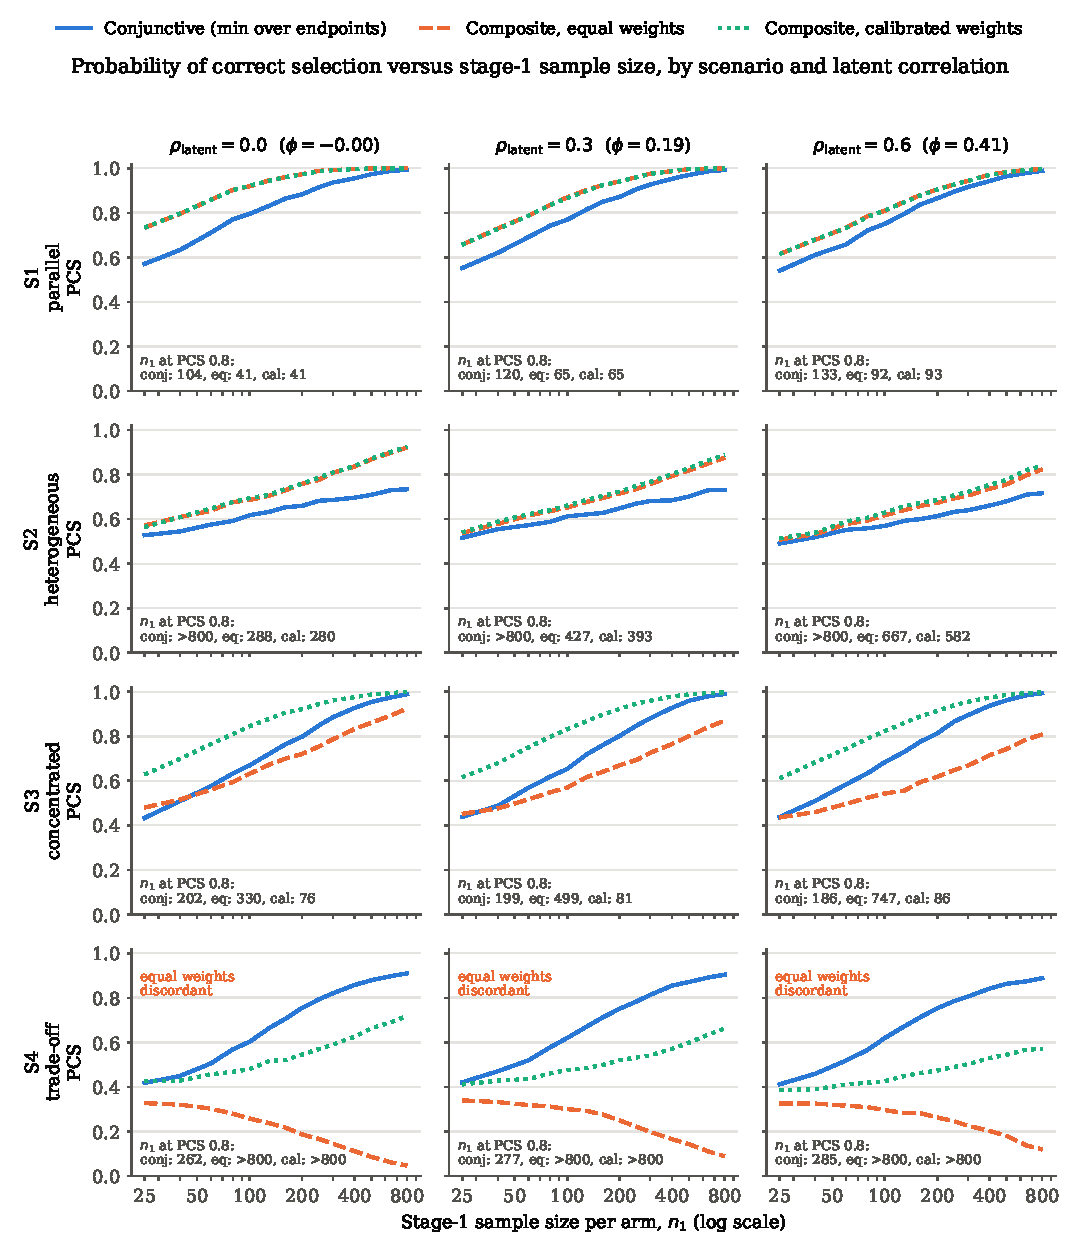
\includegraphics[width=\textwidth]{sim_fig.pdf}
\caption{Probability of correct selection against stage-1 size per arm, by configuration and latent correlation, with the target of $0.8$ marked.}\label{fig:pcs}
\end{figure}

\begin{table}
\centering\footnotesize
\caption{Stage-1 sizes at a PCS of $0.8$ by number of doses $M$, with parallel effects $0.05a$ of dose $a$ on every endpoint, $\rho=0.3$ and uniform weights.}\label{tab:msweep}
%% Generated by R/make_tables.R from results/*.csv. Do not edit by hand.
\begin{tabular}{ccccc}
\toprule
$M$ & $n_1^{\mathrm{M}}$ & $n_1^{\mathrm{C}}$ & Ratio & $\Delta N$ \\
\midrule
2 & 99 (3.6) & 56 (1.9) & 0.56 & 43 \\
3 & 106 (3.0) & 61 (2.4) & 0.58 & 90 \\
4 & 103 (3.3) & 60 (1.8) & 0.58 & 128 \\
5 & 95 (2.1) & 58 (1.3) & 0.61 & 150 \\
\bottomrule
\end{tabular}

\end{table}

\subsubsection{Stage-1 size}
Table~\ref{tab:main} and Figure~\ref{fig:pcs} give the stage-1 size at which each gate reaches a PCS of $0.8$. In S1 the composite gate needs 44--73\% of the co-primary stage-1 size, and the ratio lies inside the bracket \eqref{eq:bracket} at each correlation. The saving shrinks as the correlation grows, because the composite then averages less independent information. In S2 the co-primary gate does not reach the target within 800 subjects per arm. The composite pools a separation of $0.0175$ across endpoints and reaches the target at 283--618 with uniform weights and 289--546 with configuration-specific weights. In S3 uniform weights dilute the signal on endpoint 1 and the composite needs 1.8 to 4.2 times the co-primary size. Configuration-specific weights put 0.9--1.0 on endpoint 1 and bring the ratio to 0.44--0.46. In S4 uniform weights are discordant and the PCS falls as $n_1$ grows. Configuration-specific weights are concordant with a margin of about $0.01$ on the composite scale, and the composite does not reach the target within the grid, whereas the co-primary gate reaches it at 261--269. The ratio is stable in $M$ (Table~\ref{tab:msweep}, 0.56--0.61), and the saving $\Delta N=(M-1)(n_1^{\mathrm{M}}-n_1^{\mathrm{C}})$ grows with $M-1$.

\begin{table}
\centering\footnotesize
\caption{Jointly calibrated weights over a scenario set $\Theta$ ($n_1=100$, $\rho=0.3$), with the mean PCS over $\Theta$ of the composite and co-primary gates.}\label{tab:wjoint}
%% Generated by R/make_tables.R from results/*.csv. Do not edit by hand.
\begin{tabular}{lcccccc}
\toprule
& \multicolumn{4}{c}{$\bw^\star$} & \multicolumn{2}{c}{Mean PCS over $\Theta$} \\
\cmidrule(lr){2-5}\cmidrule(lr){6-7}
Scenario set $\Theta$ (constraint) & $w_1$ & $w_2$ & $w_3$ & $w_4$ & composite $\bw^\star$ & co-primary gate \\
\midrule
$\Theta_{\mathrm{all}}=\{$S1, S2, S3, S4$\}$ & 0.50 & 0.10 & 0.00 & 0.40 & 0.651 & 0.665 \\
$\Theta_{\mathrm{conc}}=\{$S1, S2, S3$\}$ & 0.50 & 0.20 & 0.10 & 0.20 & 0.742 & 0.684 \\
$\Theta_{\mathrm{all}}$, $w_k\ge0.10$ & 0.40 & 0.10 & 0.10 & 0.40 & 0.645 & 0.665 \\
$\Theta_{\mathrm{conc}}$, $w_k\ge0.10$ & 0.50 & 0.20 & 0.10 & 0.20 & 0.742 & 0.684 \\
\bottomrule
\end{tabular}

\end{table}

\begin{table}
\centering\footnotesize
\caption{PCS and expected regret at $n_1=100$ and $\rho=0.3$ for the co-primary gate and for the composite gate with each weight vector.}\label{tab:cross}
%% Generated by R/make_tables.R from results/*.csv. Do not edit by hand.
\setlength{\tabcolsep}{3pt}
\begin{tabular}{llccccccc}
\toprule
& & \multicolumn{1}{c}{Co-primary} & \multicolumn{6}{c}{Composite gate, weights} \\
\cmidrule(lr){3-3}\cmidrule(lr){4-9}
Configuration & & gate & uniform & $\bw^\star(\Theta_{\mathrm{all}})$ & $\bw^\star(\Theta_{\mathrm{conc}})$ & $\bw^\star(\Theta_{\mathrm{all}}, w_k\ge0.1)$ & $\bw^\star$(S3) & $\bw^\star$(S4) \\
\midrule
S1 parallel & PCS & 0.789 & 0.868 & 0.827 & 0.845 & 0.843 & 0.732 & 0.848 \\
 & regret $\times100$ & 1.17 & 0.69 & 0.94 & 0.83 & 0.84 & 1.58 & 0.81 \\
S2 heterogeneous & PCS & 0.588 & 0.650 & 0.643 & 0.647 & 0.646 & 0.581 & 0.650 \\
 & regret $\times100$ & 0.58 & 0.39 & 0.44 & 0.42 & 0.42 & 0.78 & 0.39 \\
S3 concentrated & PCS & 0.676 & 0.568 & 0.715 & 0.733 & 0.668 & 0.828 & 0.506 \\
 & regret $\times100$ & 2.65 & 3.98 & 2.37 & 2.18 & 2.86 & 1.30 & 4.74 \\
S4 trade-off & PCS & 0.607 & 0.294 & 0.419 & 0.256 & 0.423 & 0.187 & 0.457 \\
 & regret $\times100$ & 2.00 & 6.64 & 4.14 & 7.10 & 4.18 & 7.91 & 2.80 \\
\midrule
Mean PCS, S1--S4 &  & 0.665 & 0.595 & 0.651 & 0.620 & 0.645 & 0.582 & 0.615 \\
Mean PCS, S1--S3 &  & 0.684 & 0.695 & 0.728 & 0.742 & 0.719 & 0.713 & 0.668 \\
\bottomrule
\end{tabular}

\end{table}

\subsubsection{Jointly calibrated weights}
Tables~\ref{tab:wjoint} and~\ref{tab:cross} show what calibration achieves for a designer who does not know $\bm\theta$. On S1 and S2 every weight vector except $\bw^\star(\mathrm{S3})$ beats the co-primary gate on PCS and regret. On S3 the two jointly calibrated vectors and $\bw^\star(\mathrm{S3})$ beat it, and uniform weights, $\bw^\star(\mathrm{S4})$ and the floored $\bw^\star(\Theta_{\mathrm{all}})$ do not (PCS $0.568$, $0.506$ and $0.668$ against $0.676$). S4 is lost for every weight vector. Even $\bw^\star(\mathrm{S4})$ reaches a PCS of $0.46$ against $0.61$ for the co-primary gate, with $40$\% more regret. The composite must separate doses 2 and 3 by a margin of $0.01$ on the composite scale, and the co-primary gate separates them by $0.10$ on endpoint 4.

Joint calibration over a set that contains S4 gives $\bw^\star(\Theta_{\mathrm{all}})=(0.50,0.10,0.00,0.40)$. Its mean PCS over S1--S4 is $0.651$ against $0.665$ for the co-primary gate, because its gain on S1--S3 ($0.73$ against $0.68$) does not cover its loss on S4. The floor moves this vector to $(0.40,0.10,0.10,0.40)$ at a cost of $0.006$ in mean PCS, and the floored vector loses to the co-primary gate on S3 as well as S4. Calibration over the concordant set gives $\bw^\star(\Theta_{\mathrm{conc}})=(0.50,0.20,0.10,0.20)$, which already satisfies the floor. It is concordant on S1--S3 and beats the co-primary gate on each of them on both measures (PCS $0.845$, $0.647$ and $0.733$ against $0.789$, $0.588$ and $0.676$), with a PCS of $0.26$ on S4. We call $\bw^\star(\Theta_{\mathrm{conc}})$ the rule-selected weights, because the rule of Section~\ref{sec:rule} selects it for $\Theta_{\mathrm{conc}}$ and retains the co-primary gate for $\Theta_{\mathrm{all}}$. The calibrated vectors come from $2{,}000$ trials per configuration and a grid of step $0.05$, so the difference between $\bw^\star(\Theta_{\mathrm{all}})$ and its floored version is within the resolution of the calibration. The composite gate is the better selector when the plausible configurations are concordant, and the co-primary gate when a trade-off between endpoints is plausible.

\begin{table}
\centering\footnotesize
\caption{Agreement between the composite and the co-primary criterion on stage-1 data at $n_1=100$.}\label{tab:assoc}
%% Generated by R/make_tables.R from results/*.csv. Do not edit by hand.
\setlength{\tabcolsep}{3.5pt}
\begin{tabular}{lllcccccccc}
\toprule
& & & \multicolumn{4}{c}{Ranking of the $M$ doses at the interim} & \multicolumn{4}{c}{Selected dose: interim statistic and final claim} \\
\cmidrule(lr){4-7}\cmidrule(lr){8-11}
Configuration & $\rho$ & Weights & $r(z^{\mathrm{C}},z^{\mathrm{M}})$ & $\tau$ & same dose & both $a^\circ$ & $r(G,G^{\mathrm{M}})$ & AUC($G$) & AUC($G^{\mathrm{M}}$) & AUC, M gate \\
\midrule
S1 parallel & 0.0 & uniform $\mathbf w$ & 0.83 & 0.76 & 0.81 & 0.76 & 0.29 & 0.71 & 0.70 & 0.73 \\
 &  & $\mathbf w^\star(\Theta_{\mathrm{conc}})$ & 0.78 & 0.74 & 0.80 & 0.74 & 0.37 & 0.69 & 0.72 & 0.73 \\
 & 0.3 & uniform $\mathbf w$ & 0.89 & 0.78 & 0.83 & 0.74 & 0.51 & 0.73 & 0.72 & 0.75 \\
 &  & $\mathbf w^\star(\Theta_{\mathrm{conc}})$ & 0.84 & 0.75 & 0.81 & 0.72 & 0.51 & 0.72 & 0.73 & 0.75 \\
 & 0.6 & uniform $\mathbf w$ & 0.93 & 0.80 & 0.85 & 0.71 & 0.69 & 0.77 & 0.76 & 0.76 \\
 &  & $\mathbf w^\star(\Theta_{\mathrm{conc}})$ & 0.90 & 0.79 & 0.84 & 0.71 & 0.66 & 0.75 & 0.75 & 0.76 \\
\addlinespace[3pt]
S2 heterogeneous & 0.0 & uniform $\mathbf w$ & 0.81 & 0.70 & 0.71 & 0.52 & 0.31 & 0.69 & 0.69 & 0.71 \\
 &  & $\mathbf w^\star(\Theta_{\mathrm{conc}})$ & 0.75 & 0.68 & 0.70 & 0.49 & 0.35 & 0.67 & 0.69 & 0.71 \\
 & 0.3 & uniform $\mathbf w$ & 0.86 & 0.72 & 0.75 & 0.51 & 0.46 & 0.71 & 0.71 & 0.73 \\
 &  & $\mathbf w^\star(\Theta_{\mathrm{conc}})$ & 0.82 & 0.71 & 0.74 & 0.50 & 0.48 & 0.70 & 0.71 & 0.73 \\
 & 0.6 & uniform $\mathbf w$ & 0.91 & 0.76 & 0.79 & 0.52 & 0.64 & 0.72 & 0.73 & 0.75 \\
 &  & $\mathbf w^\star(\Theta_{\mathrm{conc}})$ & 0.88 & 0.75 & 0.79 & 0.51 & 0.61 & 0.72 & 0.73 & 0.75 \\
\addlinespace[3pt]
S3 concentrated & 0.0 & uniform $\mathbf w$ & 0.68 & 0.53 & 0.66 & 0.49 & 0.20 & 0.65 & 0.75 & 0.70 \\
 &  & $\mathbf w^\star(\Theta_{\mathrm{conc}})$ & 0.84 & 0.69 & 0.75 & 0.60 & 0.43 & 0.73 & 0.69 & 0.70 \\
 & 0.3 & uniform $\mathbf w$ & 0.74 & 0.55 & 0.69 & 0.49 & 0.33 & 0.66 & 0.77 & 0.70 \\
 &  & $\mathbf w^\star(\Theta_{\mathrm{conc}})$ & 0.89 & 0.71 & 0.77 & 0.59 & 0.56 & 0.73 & 0.72 & 0.70 \\
 & 0.6 & uniform $\mathbf w$ & 0.80 & 0.57 & 0.71 & 0.48 & 0.46 & 0.66 & 0.80 & 0.73 \\
 &  & $\mathbf w^\star(\Theta_{\mathrm{conc}})$ & 0.92 & 0.75 & 0.82 & 0.61 & 0.70 & 0.74 & 0.75 & 0.73 \\
\addlinespace[3pt]
S4 trade-off & 0.0 & uniform $\mathbf w$ & 0.44 & 0.11 & 0.38 & 0.21 & 0.15 & 0.61 & 0.83 & 0.73 \\
 &  & $\mathbf w^\star(\Theta_{\mathrm{conc}})$ & 0.31 & 0.07 & 0.34 & 0.18 & 0.13 & 0.59 & 0.85 & 0.73 \\
 & 0.3 & uniform $\mathbf w$ & 0.54 & 0.16 & 0.43 & 0.25 & 0.27 & 0.66 & 0.86 & 0.76 \\
 &  & $\mathbf w^\star(\Theta_{\mathrm{conc}})$ & 0.44 & 0.10 & 0.37 & 0.21 & 0.21 & 0.61 & 0.86 & 0.76 \\
 & 0.6 & uniform $\mathbf w$ & 0.63 & 0.19 & 0.45 & 0.27 & 0.37 & 0.66 & 0.86 & 0.76 \\
 &  & $\mathbf w^\star(\Theta_{\mathrm{conc}})$ & 0.54 & 0.13 & 0.39 & 0.24 & 0.32 & 0.63 & 0.88 & 0.76 \\
\bottomrule
\end{tabular}

\end{table}

\subsubsection{Agreement at the interim}
The endpoint switch requires the composite to rank the doses as the co-primary criterion would. Concordance concerns the true effects, and the stage-1 data reflect it with noise. Table~\ref{tab:assoc} measures the agreement of the two criteria on $10{,}000$ simulated stage-1 data sets per cell. Its left half reports the Pearson correlation between $z^{\mathrm{C}}_a$ and $z^{\mathrm{M}}_a$ over trials and doses, the mean Kendall $\tau$ between the two rankings of the doses within a trial, and the proportions of trials in which the two gates select the same dose and in which both select $a^\circ$. In S1--S3 the two statistics are correlated ($r=0.68$--$0.93$), $\tau$ is $0.53$--$0.80$, the two gates select the same dose in $66$--$85$\% of trials, and both select $a^\circ$ in $48$--$76$\%. The correlation also reflects the differences in true effects between doses, which both statistics follow, so $\tau$ and the same-dose proportion are the better measures. Agreement rises with the correlation between endpoints. In S3 the rule-selected weights, which load on the binding endpoint, agree better with the co-primary criterion than uniform weights ($\tau$ $0.69$--$0.75$ against $0.53$--$0.57$). In S4 the agreement is low ($\tau$ $0.07$--$0.19$, the same dose in $34$--$45$\% of trials).

The right half of Table~\ref{tab:assoc} concerns the dose that the composite selects. It reports the correlation between $G$ and $G^{\mathrm{M}}$ for that dose and the area under the ROC curve (AUC) of each as a predictor of the final claim, with the AUC of the co-primary gate's statistic at its own selected dose for comparison. $G$ and $G^{\mathrm{M}}$ are moderately correlated ($r=0.20$--$0.70$ in S1--S3), because $G$ reflects the weighted average effect and $G^{\mathrm{M}}$ the weakest endpoint. In S1 and S2 the two predict the final claim equally well (AUC $0.67$--$0.77$ for $G$ and $0.69$--$0.76$ for $G^{\mathrm{M}}$, against $0.71$--$0.76$ for the co-primary gate). In S3 with uniform weights and in S4, $G^{\mathrm{M}}$ predicts better (AUC $0.75$--$0.80$ against $0.65$--$0.66$, and $0.83$--$0.88$ against $0.59$--$0.66$). The weakest endpoint is thus informative about the final claim where the composite is not, and the per-endpoint futility check uses this information.

\subsection{Error control}\label{sec:error}

\begin{table}
\centering\footnotesize
\caption{Run A in the null configurations ($n_1=100$): probability of proceeding to stage 2, false-claim rate and expected total sample size.}\label{tab:e2eN}
%% Generated by R/make_tables.R from results/*.csv. Do not edit by hand.
\setlength{\tabcolsep}{3.5pt}
\begin{tabular}{llccccccccc}
\toprule
& & \multicolumn{3}{c}{$\Pr(\text{proceed})$} & \multicolumn{3}{c}{$\Pr(\text{false claim})$} & \multicolumn{3}{c}{$\E[N]$} \\
\cmidrule(lr){3-5}\cmidrule(lr){6-8}\cmidrule(lr){9-11}
Configuration & Design & $\rho=0$ & $0.3$ & $0.6$ & $\rho=0$ & $0.3$ & $0.6$ & $\rho=0$ & $0.3$ & $0.6$ \\
\midrule
N0 global null & M: co-primary gate & 0.21 & 0.21 & 0.21 & 0.0000 & 0.0000 & 0.0001 & 503 & 505 & 503 \\
 & C: composite, uniform $\mathbf w$ & 0.20 & 0.21 & 0.20 & 0.0000 & 0.0000 & 0.0000 & 501 & 505 & 501 \\
 & C: composite, $\mathbf w^\star(\Theta_{\mathrm{all}})$ & 0.20 & 0.20 & 0.20 & 0.0000 & 0.0000 & 0.0000 & 499 & 499 & 501 \\
 & C: composite, $\mathbf w^\star(\Theta_{\mathrm{conc}})$ & 0.20 & 0.21 & 0.20 & 0.0000 & 0.0000 & 0.0000 & 500 & 505 & 501 \\
 & C: composite, $\mathbf w^\star$(S3) & 0.20 & 0.20 & 0.20 & 0.0000 & 0.0000 & 0.0001 & 502 & 500 & 500 \\
 & C: composite, $\mathbf w^\star$(S4) & 0.20 & 0.19 & 0.20 & 0.0000 & 0.0000 & 0.0000 & 499 & 497 & 500 \\
 & C: uniform $\mathbf w$ + per-endpoint check & 0.16 & 0.20 & 0.19 & 0.0000 & 0.0000 & 0.0000 & 478 & 500 & 496 \\
 & C: $\mathbf w^\star(\Theta_{\mathrm{conc}})$ + per-endpoint check & 0.15 & 0.20 & 0.20 & 0.0000 & 0.0000 & 0.0001 & 473 & 498 & 500 \\
\addlinespace[3pt]
N1 endpoint-4 null & M: co-primary gate & 0.71 & 0.64 & 0.55 & 0.0059 & 0.0078 & 0.0103 & 754 & 719 & 676 \\
 & C: composite, uniform $\mathbf w$ & 0.98 & 0.93 & 0.86 & 0.0066 & 0.0084 & 0.0109 & 890 & 864 & 830 \\
 & C: composite, $\mathbf w^\star(\Theta_{\mathrm{all}})$ & 0.81 & 0.74 & 0.69 & 0.0061 & 0.0086 & 0.0112 & 806 & 772 & 747 \\
 & C: composite, $\mathbf w^\star(\Theta_{\mathrm{conc}})$ & 0.97 & 0.92 & 0.86 & 0.0063 & 0.0087 & 0.0111 & 883 & 858 & 832 \\
 & C: composite, $\mathbf w^\star$(S3) & 0.84 & 0.85 & 0.85 & 0.0050 & 0.0068 & 0.0088 & 822 & 823 & 824 \\
 & C: composite, $\mathbf w^\star$(S4) & 0.76 & 0.68 & 0.62 & 0.0063 & 0.0088 & 0.0114 & 782 & 740 & 711 \\
 & C: uniform $\mathbf w$ + per-endpoint check & 0.54 & 0.59 & 0.61 & 0.0057 & 0.0079 & 0.0103 & 672 & 695 & 703 \\
 & C: $\mathbf w^\star(\Theta_{\mathrm{conc}})$ + per-endpoint check & 0.54 & 0.58 & 0.60 & 0.0065 & 0.0083 & 0.0111 & 668 & 689 & 700 \\
\addlinespace[3pt]
N2 doses 1-2 null & M: co-primary gate & 0.95 & 0.93 & 0.89 & 0.0000 & 0.0000 & 0.0000 & 877 & 864 & 844 \\
 & C: composite, uniform $\mathbf w$ & 1.00 & 0.98 & 0.94 & 0.0000 & 0.0000 & 0.0000 & 899 & 891 & 870 \\
 & C: composite, $\mathbf w^\star(\Theta_{\mathrm{all}})$ & 0.97 & 0.94 & 0.91 & 0.0000 & 0.0000 & 0.0000 & 887 & 872 & 853 \\
 & C: composite, $\mathbf w^\star(\Theta_{\mathrm{conc}})$ & 0.99 & 0.96 & 0.93 & 0.0000 & 0.0000 & 0.0000 & 895 & 882 & 863 \\
 & C: composite, $\mathbf w^\star$(S3) & 0.79 & 0.79 & 0.79 & 0.0000 & 0.0000 & 0.0000 & 795 & 794 & 794 \\
 & C: composite, $\mathbf w^\star$(S4) & 0.99 & 0.96 & 0.92 & 0.0000 & 0.0000 & 0.0000 & 895 & 881 & 861 \\
 & C: uniform $\mathbf w$ + per-endpoint check & 0.95 & 0.95 & 0.93 & 0.0000 & 0.0000 & 0.0000 & 875 & 874 & 864 \\
 & C: $\mathbf w^\star(\Theta_{\mathrm{conc}})$ + per-endpoint check & 0.95 & 0.95 & 0.92 & 0.0000 & 0.0000 & 0.0000 & 873 & 873 & 861 \\
\addlinespace[3pt]
N3 staggered null & M: co-primary gate & 0.88 & 0.80 & 0.69 & 0.0167 & 0.0208 & 0.0207 & 839 & 799 & 745 \\
 & C: composite, uniform $\mathbf w$ & 1.00 & 0.98 & 0.95 & 0.0135 & 0.0154 & 0.0179 & 899 & 891 & 874 \\
 & C: composite, $\mathbf w^\star(\Theta_{\mathrm{all}})$ & 0.99 & 0.98 & 0.96 & 0.0103 & 0.0131 & 0.0146 & 897 & 890 & 880 \\
 & C: composite, $\mathbf w^\star(\Theta_{\mathrm{conc}})$ & 0.99 & 0.97 & 0.94 & 0.0105 & 0.0149 & 0.0176 & 896 & 887 & 872 \\
 & C: composite, $\mathbf w^\star$(S3) & 0.90 & 0.90 & 0.90 & 0.0097 & 0.0121 & 0.0136 & 850 & 851 & 852 \\
 & C: composite, $\mathbf w^\star$(S4) & 1.00 & 0.98 & 0.96 & 0.0118 & 0.0150 & 0.0181 & 898 & 892 & 881 \\
 & C: uniform $\mathbf w$ + per-endpoint check & 0.63 & 0.67 & 0.70 & 0.0115 & 0.0156 & 0.0172 & 714 & 736 & 749 \\
 & C: $\mathbf w^\star(\Theta_{\mathrm{conc}})$ + per-endpoint check & 0.57 & 0.61 & 0.64 & 0.0100 & 0.0137 & 0.0147 & 684 & 705 & 722 \\
\addlinespace[3pt]
N4 staggered null, large effects & M: co-primary gate & 0.90 & 0.82 & 0.70 & 0.0256 & 0.0239 & 0.0257 & 851 & 811 & 752 \\
 & C: composite, uniform $\mathbf w$ & 1.00 & 1.00 & 1.00 & 0.0176 & 0.0200 & 0.0199 & 900 & 900 & 900 \\
 & C: composite, $\mathbf w^\star(\Theta_{\mathrm{all}})$ & 1.00 & 1.00 & 1.00 & 0.0135 & 0.0148 & 0.0159 & 900 & 900 & 900 \\
 & C: composite, $\mathbf w^\star(\Theta_{\mathrm{conc}})$ & 1.00 & 1.00 & 1.00 & 0.0152 & 0.0144 & 0.0186 & 900 & 900 & 900 \\
 & C: composite, $\mathbf w^\star$(S3) & 1.00 & 1.00 & 1.00 & 0.0126 & 0.0135 & 0.0170 & 899 & 899 & 899 \\
 & C: composite, $\mathbf w^\star$(S4) & 1.00 & 1.00 & 1.00 & 0.0142 & 0.0167 & 0.0190 & 900 & 900 & 900 \\
 & C: uniform $\mathbf w$ + per-endpoint check & 0.64 & 0.67 & 0.70 & 0.0163 & 0.0168 & 0.0194 & 721 & 735 & 750 \\
 & C: $\mathbf w^\star(\Theta_{\mathrm{conc}})$ + per-endpoint check & 0.56 & 0.60 & 0.62 & 0.0127 & 0.0152 & 0.0171 & 682 & 698 & 710 \\
\bottomrule
\end{tabular}

\end{table}

\begin{table}
\centering\scriptsize
\caption{False-claim rates (N1, N3, N4) and power (S1, S3) of the full, dose-level and per-endpoint closures at $n_1=100$.}\label{tab:closure}
%% Generated by R/make_tables.R from results/*.csv. Do not edit by hand.
\setlength{\tabcolsep}{3pt}
\begin{tabular}{llccccccccc}
\toprule
& & \multicolumn{3}{c}{$\rho=0.0$} & \multicolumn{3}{c}{$\rho=0.3$} & \multicolumn{3}{c}{$\rho=0.6$} \\
\cmidrule(lr){3-5}\cmidrule(lr){6-8}\cmidrule(lr){9-11}
Configuration & Design & full & dose & endpoint & full & dose & endpoint & full & dose & endpoint \\
\midrule
N1 endpoint-4 null & M: co-primary gate & 0.0052 & 0.0088 & 0.0118 & 0.0084 & 0.0114 & 0.0142 & 0.0103 & 0.0149 & 0.0171 \\
 & C: composite, uniform $\mathbf w$ & 0.0069 & 0.0110 & 0.0140 & 0.0086 & 0.0134 & 0.0145 & 0.0112 & 0.0150 & 0.0181 \\
\addlinespace[3pt]
N3 staggered null & M: co-primary gate & 0.0176 & 0.0209 & 0.0449 & 0.0187 & 0.0228 & 0.0508 & 0.0198 & 0.0233 & 0.0459 \\
 & C: composite, uniform $\mathbf w$ & 0.0136 & 0.0144 & 0.0318 & 0.0164 & 0.0185 & 0.0366 & 0.0174 & 0.0212 & 0.0384 \\
\addlinespace[3pt]
N4 staggered null, large effects & M: co-primary gate & 0.0264 & 0.0249 & 0.0553 & 0.0241 & 0.0246 & 0.0535 & 0.0244 & 0.0246 & 0.0492 \\
 & C: composite, uniform $\mathbf w$ & 0.0180 & 0.0181 & 0.0371 & 0.0189 & 0.0195 & 0.0399 & 0.0192 & 0.0198 & 0.0410 \\
\addlinespace[3pt]
S1 parallel & M: co-primary gate & 0.656 & 0.714 & 0.738 & 0.666 & 0.730 & 0.755 & 0.681 & 0.747 & 0.753 \\
 & C: composite, uniform $\mathbf w$ & 0.718 & 0.801 & 0.822 & 0.718 & 0.788 & 0.804 & 0.713 & 0.783 & 0.792 \\
\addlinespace[3pt]
S3 concentrated & M: co-primary gate & 0.678 & 0.705 & 0.733 & 0.688 & 0.716 & 0.741 & 0.707 & 0.721 & 0.745 \\
 & C: composite, uniform $\mathbf w$ & 0.639 & 0.652 & 0.687 & 0.621 & 0.636 & 0.648 & 0.606 & 0.617 & 0.625 \\
\bottomrule
\end{tabular}

\end{table}

For every design and null configuration the false-claim rate of the full closed test is at or below $0.025$ within Monte Carlo error (Table~\ref{tab:e2eN}). The largest of the 120 estimates is $0.0257$ (N4, co-primary gate, $\rho=0.6$), one standard error above $\alpha$. Under the global null the rate is at most $0.0001$, because four null endpoints must all be rejected. In N2 at most one false claim occurred in $40{,}000$ trials, because the effective dose is almost always selected. In N1 the rates are $0.005$--$0.011$. In the staggered nulls N3 and N4 they are $0.010$--$0.026$, and the co-primary gate attains the bound in N4 ($0.024$--$0.026$). In N3 and N4 the binding intersection is the set of the three null pairs, whose stage-1 $p$-values are nearly uniform, so the closure costs little. The co-primary gate ranks each dose by the statistic of its own null endpoint. It selects the dose whose null endpoint looks best and passes a stage-1 $p$-value biased towards rejection to the final analysis. With the large effects of N4 the ranking is almost entirely a ranking of the null endpoints, and the test is at its bound. The composite gates rank on an average over endpoints and stay below it ($0.010$--$0.020$).

\begin{table}
\centering\footnotesize
\caption{False-claim rate of the full closed test with Wald $p$-values in staggered nulls, for the co-primary gate without futility stopping.}\label{tab:level}
%% Generated by R/make_tables.R from results/*.csv. Do not edit by hand.
\begin{tabular}{lcccc}
\toprule
Configuration & $n_1$ & $n_{\mathrm{tot}}$ & $\rho$ & False-claim rate (s.e.) \\
\midrule
N4 (staggered null, effects $0.25$) & 100 & 350 & 0.3 & 0.0240 (0.0003) \\
Staggered null, effects $0.35$ & 100 & 350 & 0.0 & 0.0261 (0.0004) \\
Staggered null, effects $0.35$ & 200 & 350 & 0.0 & 0.0254 (0.0004) \\
Staggered null, effects $0.35$ & 40 & 120 & 0.0 & 0.0265 (0.0004) \\
\bottomrule
\end{tabular}

\end{table}

Where the test is at its bound, the finite-sample size of the Wald test becomes visible. The one-sided Wald test of two proportions at nominal level $0.025$ has size $0.026$--$0.028$ for two arms of $40$ to $250$ subjects with a common success probability of $0.43$ or $0.50$ (two million pairs of binomial counts per cell). Table~\ref{tab:level} isolates the effect for the co-primary gate with the futility rule switched off and $200{,}000$ trials per cell. In N4 the rate is $0.0240$. When the three non-null effects are raised from $0.25$ to $0.35$, so that the stage-1 ranking is a ranking of the null endpoints alone, the rate is $0.0254$--$0.0265$, up to $0.0015$ above $\alpha$. The excess belongs to the Wald test. An exact or size-corrected test of each comparison would remove it at some cost in power.

Table~\ref{tab:closure} compares the three closures of Section~\ref{sec:final}. In N1 all three are below $\alpha$ ($0.005$--$0.018$). In N3 and N4 the per-endpoint closure gives false-claim rates of $0.045$--$0.055$ with the co-primary gate and $0.032$--$0.041$ with the composite gate, about twice and $1.3$--$1.6$ times the nominal level. The co-primary gate inflates more because its ranking statistic for each dose is nearly the statistic of that dose's null endpoint. The full closure keeps the rate at $0.014$--$0.026$ and the dose-level closure at $0.014$--$0.025$. Control in every configuration costs power. In S1 the full closure has power $0.66$--$0.68$ with the co-primary gate and $0.71$--$0.72$ with the composite gate, against $0.74$--$0.76$ and $0.79$--$0.82$ for the invalid per-endpoint closure, a cost of $0.07$--$0.10$. The dose-level closure lies between, at $0.71$--$0.75$ and $0.78$--$0.80$. In S3 the cost is $0.02$--$0.06$ for the full closure and $0.01$--$0.04$ for the dose-level closure. The composite gate's advantage in S1 shrinks with the correlation under every closure, from $0.06$--$0.09$ at $\rho=0$ to $0.03$--$0.04$ at $\rho=0.6$.

\subsection{End-to-end operating characteristics}\label{sec:e2e}

The two designs can be compared at the same $n_1$ or at the $n_1$ that each needs. At the same $n_1$ the composite design does not lower the expected sample size. Both futility boundaries are calibrated to the same probability of proceeding under the global null, and under every alternative the composite gate with uniform or jointly calibrated weights then proceeds at least as often as the co-primary gate. By \eqref{eq:EN} its $\E[N]$ is higher, at $n_1=100$ by $0$--$4$\% in S1--S3, $2$--$11$\% in S4 and $6$--$23$\% in N1, N3 and N4 (Tables~\ref{tab:e2eN} and~\ref{tab:e2eA}). Its gain at equal $n_1$ is in PCS and power (run A). The composite lowers $\E[N]$ when each design is given the $n_1$ it needs for a target PCS (run B) or a target power (run D).

\begin{table}
\centering\footnotesize
\caption{Run A in the alternative configurations ($n_1=100$): PCS, power and expected total sample size.}\label{tab:e2eA}
%% Generated by R/make_tables.R from results/*.csv. Do not edit by hand.
\setlength{\tabcolsep}{3.5pt}
\begin{tabular}{llccccccccc}
\toprule
& & \multicolumn{3}{c}{$\rho=0.0$} & \multicolumn{3}{c}{$\rho=0.3$} & \multicolumn{3}{c}{$\rho=0.6$} \\
\cmidrule(lr){3-5}\cmidrule(lr){6-8}\cmidrule(lr){9-11}
Configuration & Design & PCS & Power & $\E[N]$ & PCS & Power & $\E[N]$ & PCS & Power & $\E[N]$ \\
\midrule
S1 parallel & M: co-primary gate & 0.80 & 0.64 & 888 & 0.79 & 0.67 & 879 & 0.78 & 0.67 & 865 \\
 & C: composite, uniform $\mathbf w$ & 0.92 & 0.73 & 900 & 0.87 & 0.72 & 893 & 0.82 & 0.72 & 881 \\
 & C: composite, $\mathbf w^\star(\Theta_{\mathrm{all}})$ & 0.86 & 0.69 & 893 & 0.82 & 0.69 & 882 & 0.80 & 0.70 & 868 \\
 & C: composite, $\mathbf w^\star(\Theta_{\mathrm{conc}})$ & 0.89 & 0.70 & 898 & 0.84 & 0.69 & 888 & 0.81 & 0.70 & 874 \\
 & C: uniform $\mathbf w$ + per-endpoint check & 0.92 & 0.70 & 874 & 0.87 & 0.70 & 879 & 0.81 & 0.71 & 874 \\
 & C: $\mathbf w^\star(\Theta_{\mathrm{conc}})$ + per-endpoint check & 0.88 & 0.68 & 873 & 0.85 & 0.69 & 878 & 0.81 & 0.70 & 871 \\
\addlinespace[3pt]
S2 heterogeneous & M: co-primary gate & 0.61 & 0.37 & 882 & 0.58 & 0.41 & 865 & 0.58 & 0.45 & 846 \\
 & C: composite, uniform $\mathbf w$ & 0.69 & 0.41 & 900 & 0.65 & 0.44 & 892 & 0.63 & 0.47 & 876 \\
 & C: composite, $\mathbf w^\star(\Theta_{\mathrm{all}})$ & 0.66 & 0.38 & 890 & 0.64 & 0.43 & 878 & 0.63 & 0.46 & 863 \\
 & C: composite, $\mathbf w^\star(\Theta_{\mathrm{conc}})$ & 0.68 & 0.39 & 896 & 0.65 & 0.43 & 884 & 0.62 & 0.47 & 868 \\
 & C: uniform $\mathbf w$ + per-endpoint check & 0.69 & 0.38 & 852 & 0.64 & 0.42 & 862 & 0.63 & 0.47 & 863 \\
 & C: $\mathbf w^\star(\Theta_{\mathrm{conc}})$ + per-endpoint check & 0.67 & 0.38 & 850 & 0.66 & 0.43 & 860 & 0.62 & 0.46 & 857 \\
\addlinespace[3pt]
S3 concentrated & M: co-primary gate & 0.68 & 0.68 & 893 & 0.69 & 0.69 & 886 & 0.69 & 0.71 & 874 \\
 & C: composite, uniform $\mathbf w$ & 0.62 & 0.64 & 900 & 0.57 & 0.62 & 899 & 0.53 & 0.59 & 894 \\
 & C: composite, $\mathbf w^\star(\Theta_{\mathrm{all}})$ & 0.75 & 0.73 & 895 & 0.71 & 0.71 & 886 & 0.67 & 0.68 & 873 \\
 & C: composite, $\mathbf w^\star(\Theta_{\mathrm{conc}})$ & 0.78 & 0.75 & 898 & 0.73 & 0.73 & 891 & 0.70 & 0.71 & 882 \\
 & C: composite, $\mathbf w^\star$(S3) & 0.83 & 0.65 & 787 & 0.83 & 0.67 & 791 & 0.83 & 0.67 & 789 \\
 & C: uniform $\mathbf w$ + per-endpoint check & 0.62 & 0.64 & 864 & 0.57 & 0.61 & 866 & 0.54 & 0.60 & 867 \\
 & C: $\mathbf w^\star(\Theta_{\mathrm{conc}})$ + per-endpoint check & 0.80 & 0.74 & 884 & 0.74 & 0.73 & 885 & 0.69 & 0.71 & 879 \\
\addlinespace[3pt]
S4 trade-off & M: co-primary gate & 0.60 & 0.13 & 857 & 0.61 & 0.18 & 830 & 0.63 & 0.22 & 788 \\
 & C: composite, uniform $\mathbf w$ & 0.27 & 0.07 & 899 & 0.29 & 0.09 & 891 & 0.30 & 0.12 & 872 \\
 & C: composite, $\mathbf w^\star(\Theta_{\mathrm{all}})$ & 0.42 & 0.09 & 870 & 0.43 & 0.13 & 852 & 0.42 & 0.16 & 832 \\
 & C: composite, $\mathbf w^\star(\Theta_{\mathrm{conc}})$ & 0.23 & 0.06 & 896 & 0.27 & 0.08 & 887 & 0.27 & 0.11 & 873 \\
 & C: composite, $\mathbf w^\star$(S4) & 0.49 & 0.12 & 876 & 0.45 & 0.15 & 852 & 0.44 & 0.19 & 825 \\
 & C: uniform $\mathbf w$ + per-endpoint check & 0.26 & 0.06 & 691 & 0.29 & 0.10 & 716 & 0.31 & 0.12 & 732 \\
 & C: $\mathbf w^\star(\Theta_{\mathrm{conc}})$ + per-endpoint check & 0.23 & 0.05 & 672 & 0.26 & 0.08 & 696 & 0.27 & 0.11 & 712 \\
\bottomrule
\end{tabular}

\end{table}

\subsubsection{Run A: equal \texorpdfstring{$n_1$}{n1}}
In S1 the uniform composite raises the PCS from $0.78$--$0.80$ to $0.82$--$0.92$ and the power from $0.64$--$0.67$ to $0.72$--$0.73$, at an $\E[N]$ higher by $1$--$2$\% (Table~\ref{tab:e2eA}). The rule-selected weights keep more than half of that gain (PCS $0.81$--$0.89$, power $0.69$--$0.70$) and $\bw^\star(\Theta_{\mathrm{all}})$ about half (PCS $0.80$--$0.86$, power $0.69$--$0.70$). In S2 every design has low power at $n_{\mathrm{tot}}=350$ ($0.37$--$0.47$). The composite's PCS is $0.62$--$0.69$ against $0.58$--$0.61$, and its power is higher by $0.01$--$0.05$. In S3 uniform weights lose on PCS and power. The rule-selected weights beat the co-primary design on both (PCS $0.70$--$0.78$ against $0.68$--$0.69$, power $0.71$--$0.75$ against $0.68$--$0.71$), by a margin that shrinks with the correlation. $\bw^\star(\Theta_{\mathrm{all}})$ is better at $\rho\le0.3$ and slightly worse at $\rho=0.6$ (PCS $0.67$--$0.75$, power $0.68$--$0.73$). The single-endpoint $\bw^\star(\mathrm{S3})$ raises the PCS to $0.83$, but it proceeds in $78$\% of trials against $95$--$99$\% for the co-primary gate, whose go decision benefits from the large effects on endpoints 2--4. Its $\E[N]$ is therefore $10$--$12$\% lower and its power $0.02$--$0.04$ lower ($0.65$--$0.67$ against $0.68$--$0.71$). In S4 the co-primary design is better on every measure. Uniform and rule-selected weights are discordant there, and the two vectors calibrated on a set containing S4 are concordant by a small margin (PCS $0.23$--$0.49$ against $0.60$--$0.63$). Power is low for every design in S4 ($0.05$--$0.22$), because the optimal dose has a binding effect of only $0.08$, and dose 3, which the composite favours, is null on endpoint 4. A claim on dose 3 is a false claim, and its rate is at most $0.003$.

\subsubsection{Run A: the per-endpoint check}
In N1 the co-primary gate proceeds in $55$--$71$\% of trials, the uniform composite in $86$--$98$\%, the rule-selected composite in $86$--$97$\% and $\bw^\star(\Theta_{\mathrm{all}})$ in $69$--$81$\% (Table~\ref{tab:e2eN}). The composite design thus spends the stage-2 sample more often when one endpoint is inert ($\E[N]$ of $830$--$890$ against $676$--$754$ with uniform weights). With the check the composite proceeds in $54$--$61$\% of N1 trials with uniform weights and $54$--$60$\% with rule-selected weights. Its $\E[N]$ falls to $668$--$703$, below the co-primary design's at $\rho\le0.3$ and $4$\% above it at $\rho=0.6$. In N3 and N4 the check lowers the composite's probability of proceeding from $0.94$--$1.00$ to $0.56$--$0.70$. In S4 it lowers $\E[N]$ by $16$--$25$\% ($672$--$732$ against $872$--$899$), because the composite usually selects dose 3 there, which is negative on endpoint 4. The check costs the uniform composite $0.015$--$0.030$ of power in S1 and up to $0.03$ in S2, with the larger costs at $\rho=0$, where the check is stricter than its target, and $0.01$ or less in S3 and S4. It costs the rule-selected composite at most $0.017$, and $0.007$ or less at $\rho\ge0.3$.

\begin{table}
\centering\footnotesize
\caption{Sensitivity to the probability of proceeding under the global null to which $\eta$ is calibrated ($n_1=100$, $\rho=0.3$).}\label{tab:eta}
%% Generated by R/make_tables.R from results/*.csv. Do not edit by hand.
\begin{tabular}{llcccccc}
\toprule
Configuration & $\Pr(\text{proceed}\mid\text{N0})$ & Design & $\eta$ & $\Pr(\text{proceed})$ & PCS & Power / false claim & $\E[N]$ \\
\midrule
S1 parallel & 0.10 & M: co-primary gate & 0.665 & 0.904 & 0.788 & 0.650 & 852 \\
 & 0.10 & C: composite, uniform $\mathbf w$ & 0.960 & 0.965 & 0.865 & 0.705 & 883 \\
 & 0.20 & M: co-primary gate & 0.556 & 0.962 & 0.785 & 0.662 & 881 \\
 & 0.20 & C: composite, uniform $\mathbf w$ & 0.906 & 0.990 & 0.869 & 0.718 & 895 \\
 & 0.30 & M: co-primary gate & 0.444 & 0.977 & 0.787 & 0.669 & 889 \\
 & 0.30 & C: composite, uniform $\mathbf w$ & 0.855 & 0.995 & 0.865 & 0.714 & 897 \\
\addlinespace[3pt]
S3 concentrated & 0.10 & M: co-primary gate & 0.665 & 0.935 & 0.683 & 0.677 & 868 \\
 & 0.10 & C: composite, $\mathbf w^\star$(S3) & 0.959 & 0.622 & 0.829 & 0.548 & 711 \\
 & 0.20 & M: co-primary gate & 0.556 & 0.972 & 0.685 & 0.693 & 886 \\
 & 0.20 & C: composite, $\mathbf w^\star$(S3) & 0.903 & 0.776 & 0.836 & 0.666 & 788 \\
 & 0.30 & M: co-primary gate & 0.444 & 0.985 & 0.688 & 0.702 & 893 \\
 & 0.30 & C: composite, $\mathbf w^\star$(S3) & 0.843 & 0.851 & 0.822 & 0.705 & 826 \\
\addlinespace[3pt]
N1 endpoint-4 null & 0.10 & M: co-primary gate & 0.665 & 0.485 & 0.193 & 0.0073 & 642 \\
 & 0.10 & C: composite, uniform $\mathbf w$ & 0.960 & 0.838 & 0.027 & 0.0084 & 819 \\
 & 0.20 & M: co-primary gate & 0.556 & 0.637 & 0.196 & 0.0080 & 719 \\
 & 0.20 & C: composite, uniform $\mathbf w$ & 0.906 & 0.930 & 0.025 & 0.0085 & 865 \\
 & 0.30 & M: co-primary gate & 0.444 & 0.719 & 0.199 & 0.0085 & 759 \\
 & 0.30 & C: composite, uniform $\mathbf w$ & 0.855 & 0.960 & 0.025 & 0.0088 & 880 \\
\bottomrule
\end{tabular}

\end{table}

\subsubsection{Futility target}
Table~\ref{tab:eta} repeats the S1, S3 and N1 cells with the probability of proceeding under N0 set to $0.10$ and $0.30$. In S1 the composite's advantage in PCS ($0.87$ against $0.79$) and power ($0.71$--$0.72$ against $0.65$--$0.67$) is the same at each target. In S3 the single-endpoint $\bw^\star(\mathrm{S3})$ proceeds in $62$\% of trials at target $0.10$ and $85$\% at $0.30$, against $94$--$99$\% for the co-primary gate. Its power moves from $0.55$ to $0.71$ and matches the co-primary design's ($0.70$) at the lenient target, with a lower $\E[N]$ ($826$ against $893$). A gate that uses one endpoint therefore needs a more lenient futility rule than the co-primary gate. In N1 the false-claim rate is $0.007$--$0.009$ at every target, and the probability of proceeding ranges from $0.48$ to $0.72$ for the co-primary gate and from $0.84$ to $0.96$ for the uniform composite.

\begin{table}
\centering\footnotesize
\caption{Run B: each design at the $n_1$ that gives a PCS of $0.8$ at the selection stage (Table~\ref{tab:main}).}\label{tab:e2eB}
%% Generated by R/make_tables.R from results/*.csv. Do not edit by hand.
\begin{tabular}{llcccccc}
\toprule
Configuration & $\rho$ & Design & $n_1$ & $\Pr(\text{proceed})$ & PCS & Power & $\E[N]$ \\
\midrule
S1 parallel & 0.0 & M: co-primary gate & 94 & 0.978 & 0.794 & 0.645 & 876 \\
 & 0.0 & C: composite, uniform $\mathbf w$ & 41 & 0.950 & 0.803 & 0.683 & 751 \\
 & 0.3 & M: co-primary gate & 110 & 0.969 & 0.789 & 0.663 & 905 \\
 & 0.3 & C: composite, uniform $\mathbf w$ & 63 & 0.935 & 0.801 & 0.686 & 789 \\
 & 0.6 & M: co-primary gate & 122 & 0.957 & 0.799 & 0.698 & 925 \\
 & 0.6 & C: composite, uniform $\mathbf w$ & 89 & 0.945 & 0.806 & 0.705 & 849 \\
\addlinespace[3pt]
S3 concentrated & 0.0 & M: co-primary gate & 188 & 0.999 & 0.798 & 0.779 & 1076 \\
 & 0.0 & C: composite, $\mathbf w^\star$(S3) & 83 & 0.720 & 0.803 & 0.601 & 716 \\
 & 0.3 & M: co-primary gate & 189 & 0.997 & 0.799 & 0.790 & 1077 \\
 & 0.3 & C: composite, $\mathbf w^\star$(S3) & 84 & 0.712 & 0.811 & 0.603 & 715 \\
 & 0.6 & M: co-primary gate & 173 & 0.988 & 0.800 & 0.804 & 1042 \\
 & 0.6 & C: composite, $\mathbf w^\star$(S3) & 79 & 0.711 & 0.794 & 0.610 & 701 \\
\bottomrule
\end{tabular}

\end{table}

\subsubsection{Run B: equal PCS}
In S1, giving each design the $n_1$ at which its PCS is $0.8$ lowers the composite's $\E[N]$ by $8$--$14$\% at a power $0.01$--$0.04$ above the co-primary design (Table~\ref{tab:e2eB}). In S3 the composite with $\bw^\star(\mathrm{S3})$ reaches a PCS of $0.8$ at $n_1\approx79$--$84$. At that size the futility rule stops $28$--$29$\% of trials, and the stage-1 part of the combination test is weak. $\E[N]$ is lower by $33$--$34$\%, but power falls from $0.78$--$0.80$ to $0.60$--$0.61$. The stage-1 size also drives the futility decision and the stage-1 contribution to the final test, so $n_1$ should not be chosen from the PCS alone.

\begin{table}
\centering\footnotesize
\caption{Run C: the co-primary design (M) and the composite design with rule-selected weights (C) by $n_1$, at $n_{\mathrm{tot}}=350$ and $\rho=0.3$.}\label{tab:e2eC}
%% Generated by R/make_tables.R from results/*.csv. Do not edit by hand.
\setlength{\tabcolsep}{4pt}
\begin{tabular}{lccccccccc}
\toprule
& & \multicolumn{4}{c}{M: co-primary gate} & \multicolumn{4}{c}{C: composite gate} \\
\cmidrule(lr){3-6}\cmidrule(lr){7-10}
Configuration & $n_1$ & $\Pr(\text{proceed})$ & PCS & Power & $\E[N]$ & $\Pr(\text{proceed})$ & PCS & Power & $\E[N]$ \\
\midrule
S1 parallel & 40 & 0.767 & 0.660 & 0.518 & 635 & 0.811 & 0.710 & 0.578 & 663 \\
 & 60 & 0.884 & 0.715 & 0.607 & 753 & 0.907 & 0.771 & 0.654 & 766 \\
 & 80 & 0.922 & 0.750 & 0.633 & 818 & 0.949 & 0.806 & 0.683 & 833 \\
 & 100 & 0.961 & 0.787 & 0.662 & 881 & 0.976 & 0.842 & 0.706 & 888 \\
 & 120 & 0.975 & 0.817 & 0.679 & 929 & 0.988 & 0.869 & 0.710 & 935 \\
 & 150 & 0.989 & 0.848 & 0.685 & 996 & 0.997 & 0.897 & 0.718 & 999 \\
 & 200 & 0.997 & 0.881 & 0.705 & 1099 & 0.999 & 0.932 & 0.721 & 1100 \\
\addlinespace[3pt]
S3 concentrated & 40 & 0.839 & 0.534 & 0.528 & 680 & 0.830 & 0.606 & 0.565 & 675 \\
 & 60 & 0.916 & 0.588 & 0.600 & 771 & 0.928 & 0.659 & 0.655 & 778 \\
 & 80 & 0.951 & 0.630 & 0.644 & 833 & 0.965 & 0.707 & 0.703 & 841 \\
 & 100 & 0.974 & 0.685 & 0.701 & 887 & 0.982 & 0.733 & 0.727 & 891 \\
 & 120 & 0.980 & 0.714 & 0.728 & 931 & 0.992 & 0.764 & 0.745 & 936 \\
 & 150 & 0.990 & 0.760 & 0.759 & 996 & 0.997 & 0.802 & 0.777 & 999 \\
 & 200 & 0.996 & 0.813 & 0.798 & 1099 & 1.000 & 0.834 & 0.802 & 1100 \\
\bottomrule
\end{tabular}

\end{table}

\subsubsection{Run C: fixed \texorpdfstring{$n_{\mathrm{tot}}$}{ntot}}
Table~\ref{tab:e2eC} varies $n_1$ at $n_{\mathrm{tot}}=350$. The composite's power is higher by $0.03$--$0.06$ in S1 and $0.02$--$0.06$ in S3 for $n_1\le120$, and by $0.02$ and $0.00$ at $n_1=200$. Its $\E[N]$ is slightly higher ($888$ against $881$ in S1 and $891$ against $887$ in S3 at $n_1=100$), except at $n_1=40$ in S3 ($675$ against $680$). Power levels off at $0.71$ for the co-primary design and $0.72$ for the composite in S1, and at $0.80$ for both in S3. With $n_{\mathrm{tot}}$ fixed, the power of the closed test after a correct selection is a ceiling, and a larger $n_1$ improves selection but not confirmation. Run D removes the ceiling by varying $n_{\mathrm{tot}}$.

\begin{figure}
\centering
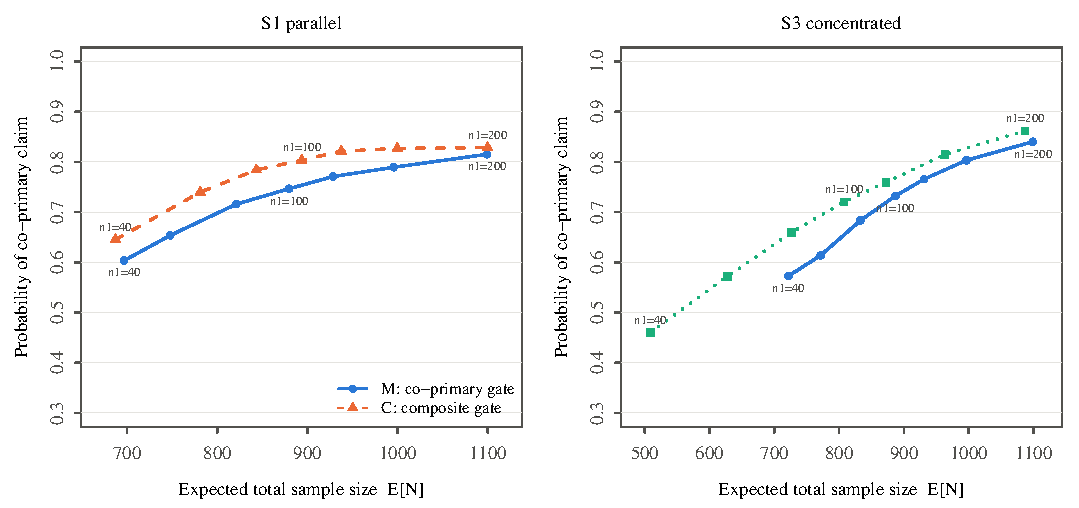
\includegraphics[width=\textwidth]{sim_e2e_fig.pdf}
\caption{Run D: smallest expected total sample size at which each design reaches a target power ($\rho=0.3$), with dotted curves for the composite designs with the per-endpoint check.}\label{fig:frontier}
\end{figure}

\begin{table}
\centering\footnotesize
\caption{Run D: the pair $(n_1,n_{\mathrm{tot}})$ with the smallest $\E[N]$ at each target power ($\rho=0.3$), with $\E[N]$ at the design alternative, under N0 and under N1 and its ratio to the co-primary design (standard errors in parentheses).}\label{tab:e2eD}
%% Generated by R/make_tables.R from results/*.csv. Do not edit by hand.
\setlength{\tabcolsep}{3.5pt}
\begin{tabular}{lllcccccccc}
\toprule
& & & & & \multicolumn{2}{c}{Design alternative} & \multicolumn{2}{c}{N0: global null} & \multicolumn{2}{c}{N1: one inert endpoint} \\
\cmidrule(lr){6-7}\cmidrule(lr){8-9}\cmidrule(lr){10-11}
Configuration & Target power & Design & $n_1$ & $n_{\mathrm{tot}}$ & $\E[N]$ & ratio to M & $\E[N]$ & ratio & $\E[N]$ & ratio \\
\midrule
S1 parallel & 0.80 & M: co-primary gate & 99 & 450 & 1067 (6) & 1 & 539 & 1 & 838 & 1 \\
 &  & C: composite, uniform $\mathbf w$ & 60 & 450 & 971 (5) & 0.91 (0.01) & 400 & 0.74 & 872 & 1.04 \\
 &  & C: composite, $\mathbf w^\star(\Theta_{\mathrm{conc}})$ & 78 & 450 & 1014 (6) & 0.95 (0.01) & 465 & 0.86 & 957 & 1.14 \\
 &  & C: uniform $\mathbf w$ + per-endpoint check & 78 & 450 & 998 (6) & 0.94 (0.01) & 465 & 0.86 & 751 & 0.90 \\
 &  & C: $\mathbf w^\star(\Theta_{\mathrm{conc}})$ + per-endpoint check & 85 & 450 & 1021 (6) & 0.96 (0.01) & 485 & 0.90 & 757 & 0.90 \\
\addlinespace[3pt]
 & 0.85 & M: co-primary gate & 109 & 500 & 1191 (7) & 1 & 595 & 1 & 936 & 1 \\
 &  & C: composite, uniform $\mathbf w$ & 90 & 450 & 1065 (6) & 0.90 (0.01) & 507 & 0.85 & 1013 & 1.08 \\
 &  & C: composite, $\mathbf w^\star(\Theta_{\mathrm{conc}})$ & 111 & 450 & 1111 (15) & 0.93 (0.01) & 582 & 0.98 & 1080 & 1.15 \\
 &  & C: uniform $\mathbf w$ + per-endpoint check & 111 & 450 & 1101 (11) & 0.92 (0.01) & 581 & 0.98 & 842 & 0.90 \\
 &  & C: $\mathbf w^\star(\Theta_{\mathrm{conc}})$ + per-endpoint check & 117 & 450 & 1114 (9) & 0.94 (0.01) & 597 & 1.00 & 848 & 0.91 \\
\addlinespace[3pt]
 & 0.90 & M: co-primary gate & 182 & 500 & 1359 (16) & 1 & 855 & 1 & 1154 & 1 \\
 &  & C: composite, uniform $\mathbf w$ & 99 & 500 & 1189 (9) & 0.88 (0.01) & 555 & 0.65 & 1136 & 0.98 \\
 &  & C: composite, $\mathbf w^\star(\Theta_{\mathrm{conc}})$ & 124 & 500 & 1239 (19) & 0.91 (0.02) & 645 & 0.75 & 1208 & 1.05 \\
 &  & C: uniform $\mathbf w$ + per-endpoint check & 120 & 500 & 1222 (11) & 0.90 (0.01) & 631 & 0.74 & 920 & 0.80 \\
 &  & C: $\mathbf w^\star(\Theta_{\mathrm{conc}})$ + per-endpoint check & 136 & 500 & 1255 (10) & 0.92 (0.01) & 697 & 0.81 & 961 & 0.83 \\
\addlinespace[3pt]
S3 concentrated & 0.80 & M: co-primary gate & 137 & 400 & 1068 (7) & 1 & 660 & 1 & 892 & 1 \\
 &  & C: composite, $\mathbf w^\star(\Theta_{\mathrm{conc}})$ & 115 & 400 & 1024 (10) & 0.96 (0.01) & 568 & 0.86 & 993 & 1.11 \\
 &  & C: composite, $\mathbf w^\star$(S3) & 149 & 400 & 1030 (7) & 0.96 (0.01) & 695 & 1.05 & 1065 & 1.19 \\
 &  & C: $\mathbf w^\star(\Theta_{\mathrm{conc}})$ + per-endpoint check & 124 & 400 & 1037 (10) & 0.97 (0.01) & 605 & 0.92 & 812 & 0.91 \\
\addlinespace[3pt]
 & 0.85 & M: co-primary gate & 194 & 400 & 1186 (10) & 1 & 862 & 1 & 1054 & 1 \\
 &  & C: composite, $\mathbf w^\star(\Theta_{\mathrm{conc}})$ & 132 & 450 & 1160 (9) & 0.98 (0.01) & 658 & 0.76 & 1138 & 1.08 \\
 &  & C: composite, $\mathbf w^\star$(S3) & 189 & 400 & 1144 (8) & 0.96 (0.01) & 841 & 0.98 & 1161 & 1.10 \\
 &  & C: $\mathbf w^\star(\Theta_{\mathrm{conc}})$ + per-endpoint check & 134 & 450 & 1158 (14) & 0.98 (0.01) & 660 & 0.77 & 895 & 0.85 \\
\addlinespace[3pt]
 & 0.90 & M: co-primary gate & 178 & 500 & 1352 (8) & 1 & 835 & 1 & 1130 & 1 \\
 &  & C: composite, $\mathbf w^\star(\Theta_{\mathrm{conc}})$ & 171 & 500 & 1340 (9) & 0.99 (0.01) & 813 & 0.97 & 1330 & 1.18 \\
 &  & C: composite, $\mathbf w^\star$(S3) & 196 & 500 & 1349 (6) & 1.00 (0.01) & 904 & 1.08 & 1370 & 1.21 \\
 &  & C: $\mathbf w^\star(\Theta_{\mathrm{conc}})$ + per-endpoint check & 169 & 500 & 1333 (12) & 0.99 (0.01) & 805 & 0.96 & 1053 & 0.93 \\
\bottomrule
\end{tabular}

\end{table}

\subsubsection{Run D: target power}
Table~\ref{tab:e2eD} and Figure~\ref{fig:frontier} treat $n_1$ and $n_{\mathrm{tot}}$ as design parameters. For each $n_{\mathrm{tot}}$ on the grid, the $n_1$ at which the power reaches the target is found by linear interpolation, and the $n_{\mathrm{tot}}$ with the smallest interpolated $\E[N]$ is taken. In S1 the uniform composite reaches the three targets with $9$--$12$\% fewer expected subjects than the co-primary design ($\E[N]$ ratios $0.91$, $0.90$ and $0.88$), and the rule-selected composite with $5$--$9$\% fewer ($0.95$, $0.93$ and $0.91$). At target $0.80$ both designs choose $n_{\mathrm{tot}}=450$, and the uniform composite needs $n_1=60$ against $99$. The saving is the stage-1 saving of Section~\ref{sec:saving} less the stage-2 subjects that the composite spends on trials it does not stop. In S3 the saving is $0$--$4$\% with $\bw^\star(\mathrm{S3})$ and $1$--$4$\% with the rule-selected weights, so the selection-stage ratio of $0.44$--$0.46$ in Table~\ref{tab:main} becomes a few per cent of $\E[N]$. The standard error of a ratio is $0.01$--$0.02$, the grid step in $n_{\mathrm{tot}}$ is $50$ or $100$ subjects per arm, and the minimum over independently simulated cells is slightly optimistic for every design. We summarise the result as a saving of about $10$\% in S1 and no material saving in S3. The per-endpoint check costs one to three points of the S1 saving (ratios $0.94$, $0.92$ and $0.90$ with uniform weights, $0.96$, $0.94$ and $0.92$ with rule-selected weights) and at most one point in S3 ($0.97$, $0.98$ and $0.99$), because the checked design proceeds less often under the alternative and chooses a slightly larger $n_1$.

The last four columns of Table~\ref{tab:e2eD} give $\E[N]$ under N0 and N1 for each design at its optimum, from $20{,}000$ trials per cell. Under N0 no composite with uniform or rule-selected weights costs more than the co-primary design (ratios $0.65$--$1.00$), because it proceeds with the same probability from a smaller stage 1. The single-endpoint $\bw^\star(\mathrm{S3})$ needs a larger $n_1$ and has ratios of $0.98$--$1.08$. Under N1 the composite without the check costs more than the co-primary design at every target but one, by $4$--$15$\% in S1 and $8$--$21$\% in S3, because it proceeds in $81$--$98$\% of trials against $63$--$68$\%. With the check it proceeds in $57$--$59$\% of trials and costs $7$--$20$\% less than the co-primary design (ratios $0.80$--$0.93$).

\subsection{Prior sensitivity}\label{sec:prior}

The prior enters only the stage-1 statistics. The final test uses Wald $p$-values, so Theorem~\ref{thm:t1e} holds for any prior. Table~\ref{tab:prior} repeats the comparison of the co-primary gate and the rule-selected composite gate in S1 and S3 at $\rho=0.3$ under five other priors. The Jeffreys prior $\Dir(\mathbf 1/2)$ and the flat prior $\Dir(\mathbf 1)$ on every arm carry the weight of $J/2=8$ and $J=16$ observations and shrink every success probability towards $0.5$. An informative prior $\Dir(m\,\mathbf q_0)$ on the control arm only, with mass $m=20$ or $50$, is centred on the true control cell probabilities $\mathbf q_0$, as historical control data might give in the most favourable case. The same prior with $m=50$ is also centred on $\tilde{\mathbf q}_0$, whose success probabilities lie $0.10$ above the truth. The column Mass gives the prior mass on a dose arm and on the control arm. The boundary $\eta$ is recalibrated for each gate and prior. The reference rows differ from Table~\ref{tab:main} (ratios $0.70$ and $0.81$ against $0.57$ and $0.44$), because that table uses uniform and configuration-specific weights.

\begin{table}
\centering\footnotesize
\caption{Prior sensitivity at $\rho=0.3$: stage-1 size at a PCS of $0.8$ and, at $n_1=100$ and $n_{\mathrm{tot}}=350$, PCS, power and $\E[N]$ for the co-primary gate (M) and the rule-selected composite gate (C).}\label{tab:prior}
%% Generated by R/make_tables.R from results/*.csv. Do not edit by hand.
\setlength{\tabcolsep}{3.5pt}
\begin{tabular}{lllccccccccc}
\toprule
& & & \multicolumn{3}{c}{$n_1$ at $\PCS=0.8$} & \multicolumn{6}{c}{$n_1=100$, $n_{\mathrm{tot}}=350$} \\
\cmidrule(lr){4-6}\cmidrule(lr){7-12}
& & & & & & \multicolumn{2}{c}{PCS} & \multicolumn{2}{c}{Power} & \multicolumn{2}{c}{$\E[N]$} \\
\cmidrule(lr){7-8}\cmidrule(lr){9-10}\cmidrule(lr){11-12}
Configuration & Prior & Mass & M & C & C/M & M & C & M & C & M & C \\
\midrule
S1 parallel & $\Dir(\mathbf 1/J)$, all arms (reference) & 1 / 1 & 110 (2) & 77 (2) & 0.70 & 0.78 & 0.84 & 0.65 & 0.70 & 876 & 888 \\
 & $\Dir(\mathbf 1/2)$, all arms & 8 / 8 & 112 (3) & 73 (2) & 0.65 & 0.79 & 0.84 & 0.67 & 0.70 & 879 & 887 \\
 & $\Dir(\mathbf 1)$, all arms & 16 / 16 & 109 (3) & 72 (1) & 0.66 & 0.80 & 0.84 & 0.67 & 0.70 & 880 & 889 \\
 & $\Dir(20\,\mathbf q_0)$ on control & 1 / 20 & 103 (4) & 75 (2) & 0.73 & 0.80 & 0.84 & 0.68 & 0.70 & 887 & 894 \\
 & $\Dir(50\,\mathbf q_0)$ on control & 1 / 50 & 97 (3) & 72 (2) & 0.75 & 0.80 & 0.85 & 0.68 & 0.71 & 894 & 898 \\
 & $\Dir(50\,\tilde{\mathbf q}_0)$ on control & 1 / 50 & 104 (3) & 72 (2) & 0.69 & 0.80 & 0.84 & 0.67 & 0.71 & 895 & 898 \\
\addlinespace[3pt]
S3 concentrated & $\Dir(\mathbf 1/J)$, all arms (reference) & 1 / 1 & 192 (4) & 156 (4) & 0.81 & 0.69 & 0.74 & 0.69 & 0.73 & 885 & 890 \\
 & $\Dir(\mathbf 1/2)$, all arms & 8 / 8 & 189 (3) & 148 (4) & 0.78 & 0.68 & 0.73 & 0.69 & 0.73 & 884 & 891 \\
 & $\Dir(\mathbf 1)$, all arms & 16 / 16 & 206 (4) & 153 (6) & 0.74 & 0.67 & 0.74 & 0.68 & 0.72 & 884 & 890 \\
 & $\Dir(20\,\mathbf q_0)$ on control & 1 / 20 & 179 (4) & 150 (3) & 0.84 & 0.69 & 0.74 & 0.70 & 0.73 & 892 & 897 \\
 & $\Dir(50\,\mathbf q_0)$ on control & 1 / 50 & 167 (3) & 157 (4) & 0.94 & 0.72 & 0.74 & 0.73 & 0.74 & 897 & 899 \\
 & $\Dir(50\,\tilde{\mathbf q}_0)$ on control & 1 / 50 & 165 (4) & 155 (5) & 0.94 & 0.71 & 0.74 & 0.72 & 0.73 & 896 & 899 \\
\bottomrule
\end{tabular}

\end{table}

The conclusions of Sections~\ref{sec:selection} and \ref{sec:e2e} hold under every prior. Across the six priors the PCS at $n_1=100$ varies by at most $0.01$ for the composite gate and by less than $0.05$ for the co-primary gate, power by at most $0.02$ and by less than $0.05$, and $\E[N]$ by about $2$\% or less. In S1 the composite reaches a PCS of $0.8$ with $25$--$35$\% fewer stage-1 subjects per arm under every prior. In S3 this stage-1 saving is $19$--$26$\% under the three exchangeable priors, $16$\% with the control prior of mass $20$ and $6$\% with mass $50$. A sharper control posterior helps the co-primary gate, because it changes which endpoint is binding for each dose, and hardly changes the composite ranking, where the control enters through a term common to all doses. These figures are stage-1 sizes, and the $\E[N]$ comparison at target power (Table~\ref{tab:e2eD}) was not repeated under other priors. The informative priors also raise the probability of proceeding under the alternative (from $0.95$ to $0.99$ for the co-primary gate in S1), which raises $\E[N]$ slightly.

Table~\ref{tab:prior} calibrates $\eta$ under the global null at the true control rates. With that calibration, centring the control prior $0.10$ too high moves $n_1$ at a PCS of $0.8$ by at most $8$ subjects per arm and the PCS and power by at most $0.012$ relative to the correctly centred prior. A designer who trusts the historical data would calibrate $\eta$ at the control rates they believe. Table~\ref{tab:prior_belief} does this for the mass-$50$ prior and runs the trial at the true rates. With a belief $0.10$ too high, power falls by about $0.01$ and the comparison of gates is unchanged, but the trial proceeds under the true global null in $3$--$4$\% of trials against the intended $20$\%. With a belief $0.10$ too low it proceeds in $54$--$56$\% of null trials, and $\E[N]$ under the null rises by a third. A wrong historical control thus changes the futility behaviour and leaves the error rate unchanged, and we recommend the weak prior unless the historical data are trusted.

\begin{table}
\centering\footnotesize
\caption{The mass-$50$ control prior with $\eta$ calibrated at the control rates the designer believes and the trial run at the true rates ($n_1=100$, $n_{\mathrm{tot}}=350$, $\rho=0.3$).}\label{tab:prior_belief}
%% Generated by R/make_tables.R from results/*.csv. Do not edit by hand.
\begin{tabular}{llcccccccc}
\toprule
& & \multicolumn{2}{c}{N0 global null} & \multicolumn{3}{c}{S1 parallel} & \multicolumn{3}{c}{S3 concentrated} \\
\cmidrule(lr){3-4}\cmidrule(lr){5-7}\cmidrule(lr){8-10}
Historical control & Gate & $\Pr(\text{proceed})$ & $\E[N]$ & PCS & Power & $\E[N]$ & PCS & Power & $\E[N]$ \\
\midrule
centred on the truth & M & 0.19 & 495 & 0.80 & 0.68 & 895 & 0.71 & 0.73 & 896 \\
 & C & 0.21 & 507 & 0.85 & 0.71 & 898 & 0.73 & 0.73 & 899 \\
\addlinespace[3pt]
optimistic ($+0.10$) & M & 0.04 & 421 & 0.80 & 0.66 & 866 & 0.72 & 0.71 & 877 \\
 & C & 0.03 & 417 & 0.84 & 0.70 & 877 & 0.74 & 0.73 & 883 \\
\addlinespace[3pt]
pessimistic ($-0.10$) & M & 0.54 & 668 & 0.80 & 0.68 & 900 & 0.71 & 0.72 & 899 \\
 & C & 0.56 & 678 & 0.84 & 0.71 & 900 & 0.74 & 0.73 & 900 \\
\bottomrule
\end{tabular}

\end{table}

\subsection{Design rule}\label{sec:rule}

For a pre-specified scenario set $\Theta$ we recommend four steps.
\begin{enumerate}[label=(\arabic*),leftmargin=*]
\item Calibrate $\bw^\star$ by \eqref{eq:weights} over $\Theta$ under the clinical constraints $\cW$ and a floor $w_k\ge w_{\min}$, so that no endpoint is ignored. Consider the composite gate only if $\bw^\star$ is concordant at every $\bm\theta\in\Theta$ and has the higher PCS at every $\bm\theta\in\Theta$ in a cross-evaluation such as Table~\ref{tab:cross}. Otherwise, as when $\Theta$ contains a trade-off configuration, retain the co-primary gate.
\item Calibrate $\eta$ for each gate, with the per-endpoint check when it is used, to a common probability of proceeding under the global null.
\item For each gate, choose the pair $(n_1,n_{\mathrm{tot}})$ with the smallest $\E[N]$ at which the design reaches the target power at the design alternative, as in Table~\ref{tab:e2eD}.
\item Adopt the composite gate only if its $\E[N]$ is below that of the co-primary gate at its own optimum. If failure on a single endpoint is plausible, add the per-endpoint check and include $\E[N]$ under that configuration in the comparison.
\end{enumerate}
The final analysis of Section~\ref{sec:final} is the same for either gate. In the vaccine example a better formulation tends to be better on every serogroup and the weights can be fixed from disease burden, so step (1) is plausible. The serogroup A shortfall observed by \citet{ostergaard2009} is the configuration that step (4) addresses.

\section{Discussion}\label{sec:disc}

A seamless phase II/III trial with co-primary endpoints selects a dose and then confirms it. The proposed design gives the two tasks to two criteria. A weighted composite selects the dose, and the co-primary test with the stage-1 data included confirms it. Theorem~\ref{thm:t1e} shows that this costs nothing in type I error if the closed test is taken over all dose--endpoint hypotheses. Closing each endpoint separately over doses, the direct extension of the single-endpoint method, does not control the false-claim rate when different doses fail on different endpoints. The dose-level closure of Appendix~\ref{app:union} is also valid. It recovers $0.7$--$0.9$ of the power that the full closure loses relative to that invalid procedure under parallel effects, and $0.3$--$0.6$ of it in the concentrated configuration (Table~\ref{tab:closure}). It suits analyses that make no per-endpoint statement about the selected dose.

The composite saves sample size under conditions. With parallel effects and uncorrelated endpoints the stage-1 size needed for selection falls by more than half. At a power of $0.80$--$0.90$ the expected total sample size falls by about $10$\%, or by $6$--$10$\% with uniform weights and $4$--$8$\% with rule-selected weights when the per-endpoint check is added. The saving comes from the smaller stage 1. When one endpoint separates the doses, the saving at target power was at most $4$\%, even with weights calibrated on that configuration. When the best dose is a trade-off between endpoints, the composite selects worse than the co-primary criterion.

Two conditions therefore decide whether the design should be used. The first is concordance, which in the vaccine setting rests on the biology of the carrier-conjugate response and on the epidemiology that fixes the weights. Calibration does not replace that knowledge: weights calibrated over a scenario set with a trade-off configuration lost to the co-primary gate on average. The second is the plausibility of failure on a single endpoint. The per-endpoint check moved the composite's $\E[N]$ under one inert endpoint from $4$--$21$\% above the co-primary design's to $7$--$20$\% below it, for one to three points of the saving under the alternative.

The study has limitations. The simulation used a latent Gaussian threshold model with one correlation, and we did not study cell probabilities with the same pairwise correlations and a different higher-order structure. The stage-2 size was fixed, although Theorem~\ref{thm:t1e} covers re-estimation. The futility boundary was calibrated to a common probability of proceeding under the global null, and other calibrations would shift the results of both designs. The simulation tested superiority, and non-inferiority changes only the margins $\delta_k$ and $\gamma$. Estimates for the selected dose from the pooled data are biased by the selection \citep{bowden2008,kimani2013}. Here the selection acts on the composite, and the bias reaches each endpoint through the cells it shares with the composite. The stage-2 data alone give estimates free of this bias, and a selection-adjusted estimator is a topic for further work.
